\documentclass[10pt,a4paper]{report}

\usepackage[T1]{fontenc}
\usepackage{titlesec, blindtext, color}
\newcommand{\hsp}{\hspace{10pt}}

\usepackage[utf8]{inputenc}
\usepackage{amsmath}
\usepackage{amsfonts}
\usepackage{amssymb}
\usepackage{enumitem}

\usepackage{caption}
\usepackage{float}
\usepackage{graphicx}
\usepackage{hyperref}
\usepackage{xcolor}

\title{
\includegraphics[scale=6.0]{App Icon}\\Requirement Specification for Graphical Editor for Liberty Files}

\author{Alp Toraç Genç, Kerem Kara, Xhulio Pernoca, Manuel Schenk, Ege Uzhan \leavevmode \\---------------------------------------------------------------------------------------\\
Submitted to: Om Prakash, Georgios Zervakis, Faeze Faghih}
\date{\today}

% Format for the chapters/sections/subsections
\titleformat{\chapter}[hang]{\Huge\bfseries}{\thechapter\hsp{}}{0pt}{\Huge\bfseries}
\titlespacing{\chapter}{0cm}{0cm}{0.5cm} % distance from {right}{left}{next line} for chapter
\titlespacing{\subsection}{0cm}{0cm}{0.5cm} % distance from {right}{left}{next line} for subsection

%Functional requirements list
\newlist{FR}{enumerate}{1}
\setlist[FR]{label=FR-\arabic*}

%Optional functional requirements list
\newlist{FRO}{enumerate}{1}
\setlist[FRO]{label=FRO-\arabic*}

%Mandatory Non-Functional requirements (reliability) list
\newlist{NFR-Rel}{enumerate}{1}
\setlist[NFR-Rel]{label=NFR-Rel-\arabic*}

%Mandatory Non-Functional requirements (performance) list
\newlist{NFR-Perf}{enumerate}{1}
\setlist[NFR-Perf]{label=NFR-Perf-\arabic*}

%Mandatory Non-Functional requirements (robustness) list
\newlist{NFR-Rob}{enumerate}{1}
\setlist[NFR-Rob]{label=NFR-Rob-\arabic*}

%Optional Non-Functional requirements (usability) list
\newlist{NFRO-Usability}{enumerate}{1}
\setlist[NFRO-Usability]{label=NFRO-Usability-\arabic*}

%Optional Non-Functional requirements (performance) list
\newlist{NFRO-Perf}{enumerate}{1}
\setlist[NFRO-Perf]{label=NFRO-Perf-\arabic*}

%Global test cases for core functional requirements
\newlist{GTC}{enumerate}{1}
\setlist[GTC]{label=+GTC-\arabic*}

%Global test cases for optional functional requirements
\newlist{GTCO}{enumerate}{1}
\setlist[GTCO]{label=+GTCO-\arabic*}

%Macro for Glossary entries
% #1: Name of the label (glo:#1)
% #2: Display in Glossary
% #3: Description
\newcommand{\itemglo}[3]{
    \label{glo:#1}\textbf{#2}
    \begin{itemize}[noitemsep, topsep=0pt, label=]
        \item #3
    \end{itemize}
}

%MACROS

% Macros for describing functional requirements/test cases
% #1: Precondition/Action/State/Reaction
\newcommand{\precondition}[1]{
    \textbf{Precondition: } #1 \leavevmode \\
}
\newcommand{\postcondition}[1]{
    \textbf{Postcondition: } #1 \leavevmode \\
}
\newcommand{\action}[1]{
    \textbf{Action: } #1 \leavevmode \\
}
\newcommand{\state}[1]{
    \textbf{State: } #1 \leavevmode \\
}
\newcommand{\reaction}[1]{
    \textbf{Reaction: } #1 \leavevmode \\
}

% Macro for describing the mandatory functional requirements
% #1: Name of the functional requirement
% #2: Goal
% #3: Importance
% #4: Precondition
% #5: Post Condition (success)
% #6: Post Condition (fail)
% #7: Triggering Event(s)
% #8: Description
\newcommand{\FRDescription}[8]{
    \textbf{#1} \leavevmode \\
    \textbf{Goal: } #2 \leavevmode \\
    \textbf{Importance: } #3 \leavevmode \\
    \precondition{#4}
    \textbf{Post Condition (success): } #5 \leavevmode \\
    \textbf{Post Condition (fail): } #6 \leavevmode \\
    \textbf{Triggering Event(s): } #7 \leavevmode \\
    \textbf{Description: } \leavevmode \\ 
    #8}
    
% Macro for describing the optional functional requirements
% #1: Name of the functional requirement
% #2: Goal
% #3: Importance
% #4: Precondition
% #5: Post Condition (success)
% #6: Post Condition (fail)
% #7: Triggering Event(s)
% #8: Description
\newcommand{\FRODescription}[8]{
    \textbf{#1} \leavevmode \\
    \textbf{Goal: } #2 \leavevmode \\
    \textbf{Importance: } #3 \leavevmode \\
    \precondition{#4}
    \textbf{Post Condition (success): } #5 \leavevmode \\
    \textbf{Post Condition (fail): } #6 \leavevmode \\
    \textbf{Triggering Event(s): } #7 \leavevmode \\
    \textbf{Description: } \leavevmode \\
    #8}

% Macro for describing global test cases for mandatory/optional functional requirements
% #1: Bullet points of functional requirements (ex: FR-1, FRO-2 and FR-5)
% #2: Name of the test case
\newcommand{\GTCDescription}[2]{
    (\textbf{Tests: #1}) \textbf{#2} \leavevmode \\
}
\newcommand{\GTCODescription}[2]{
    (\textbf{Tests: #1}) \textbf{#2} \leavevmode \\
}

% Macro for adding attributes
% #1: Name of the attribute
% #2: Description of the attribute
\newcommand{\attribute}[2]{
    #1 \leavevmode \\ #2
}

% Macro for referencing another section in the document
% #1 Name of referenced section
% #2 Text of link
\definecolor{col:reference}{HTML}{2f5399}
\newcommand{\refer}[2]{\hyperref[#1]{\textcolor{col:reference}{#2}}}

%Macro for Highlighting
% #1 Text to highlight
\definecolor{col:highlight}{HTML}{63b53e}
\newcommand{\h}[1]{\textcolor{col:highlight}{#1}}

%Macro for creating a Glossary entry
% #1 name(reference)
% #2 name(display)
% #3 description
%\newcommand{\defg}[3]{\label{glo:#1}\section{#2}#3\\}

%Macro for Interaction Type Definitions
% #1 name
% #2 interaction type
% #3 definition
\newcommand{\defit}[3]{\subsection{#2}\label{it:#1}#3}

%Macro for UI Element Definitions
% #1 name
% #2 interaction type
% #3 related functional requirement(s)
\newcommand{\ui}[3]{
    \begin{description}
        \item[Name]{#1}
        \item[Interaction]{#2}
        \item[Related FR]{#3}
    \end{description}
}

%Macro for referencing glossary entries
% 1 name of glossary entry
% 2 display text
\newcommand{\refg}[2]{\refer{glo:#1}{#2}}

% Aligns captions to the left of the images
\captionsetup{
  font=footnotesize,
  justification=raggedright,
  singlelinecheck=false
}

% Macro for including images
\newcommand{\includeimage}[5]{
    \begin{figure}[H]
        #1
        \includegraphics[scale=#2]{#3.png}
        \caption{#4}
        \label{fig:#5}
    \end{figure}
}

% Macro for adding graph images
\newcommand{\includegraph}[7]{
    \graphicspath{{#1}}
    \includeimage{#2}{#3}{#4}{#5}{#6}
    \graphicspath{{#7}}
}

\newcommand{\imagepath}{Images/}
\newcommand{\graphpath}{Images/Graphs/}

\graphicspath{\imagepath}

\begin{document}
\maketitle
\label{sec:title}
\tableofcontents

\chapter{Purpose}
\section{Product Goal}
\setlength{\parindent}{0pt}
"Liberty, when it begins to take root, is a plant of rapid growth." 

-George Washington \\


Liberty format is a text based file format where cell libraries are stored. These cell libraries can store a lot of information about components. However, the liberty files usually contain thousands of lines of text, which makes them impractical to read, to find desired values or to compare cells/pins with each other.
\\

What we aim to achieve is to make it easier for everyone to understand liberty files and also to easily make operations on them.
\\

With the help of a hierarchical display of the files the user will be able to navigate through the levels of the library easily. By using different types of statistics and visualizations it will be easier to see the behaviors of components and also to compare them with each other. GELF's(Graphical Editor for Liberty Files) way of visualizing Liberty Files by drawing complicated values in a graph makes the viewer examine different component attributes and behaviours. Instead of being forced to read thousands of lines of hard to understand text, GELF will provide the same information in a much more direct and manageable way, so that the user can work around these complicated files with ease.
\\

GELF is going to give this liberty to everyone trying to understand Liberty Files or work with them.
\section{Target Audience}
Target audience for GELF desktop app is mainly hardware and electrical engineers, who are dealing with Liberty Files. GELF can be used by anyone with a computer with Linux. It provides an easier to work environment for Liberty Files, which will help engineers to observe and examine behaviors of components. It also make it possible to compare different components by their different attributes, which would further help engineers to spot the characteristics of components and make decisions about them.
\chapter{Scenarios}
\section{Comparing Components}
\setlength{\parindent}{0em}


A portable device manufacturer aims to make their new device's battery last longer than the devices of rival companies. For that to happen the device should have the least possible amount of power leakage while in sleep mode. So they decide to compare different components by their leakage information. 
\\

They open GELF (Graphical Editor for Liberty Files) desktop app, then open two liberty files through file manager. The liberty files get displayed hierarchically in a tree view.
\\

First they select their libraries and open them in two different panels with the options of "Editor" and "View". They select "View" to visualize information about the libraries. From the drop down menu of attributes they select leakage power in both panels and a bar chart is drawn in both panels, showing the averages of leakage powers of cells in the libraries. 
\\

Then they select these two libraries from the tree view on the left and click on "Compare". A new panel opens with just "View" option for comparison. They again select leakage power and see that the two bar charts from before are put on top of each other.
\\

With a click on a name of the cell on the first two panels, the cell view is opened in the panels with images of the cells. They click on different checkboxes near pin names to change the function of cells and to see the leakage power values accordingly.
\\

They select two cells from the tree view, click on "Compare" and select leakage power. The bar charts are put on top of each other with functions of cells as indexes. At last they select 10 different cells and select default leakage value and a bar chart appears, which has a single value for each selected cell.
\\

With all the information at their hand, they decide which components would be more beneficial for them to use. They make some adjustments in the text editor and merge the libraries of components they want to use in a new file. They save the file on the computer and close the program.
\newpage
\section{A Merge Conflict}

Two PhD students make a shift register for a project. With a liberty file, they want to provide some information about the gates and other components they used to their professor. 
\\

Although they have info about their components, they are all in different liberty files, so they are in search of an easy way to bring these different components into a single library. They also want to change an internal power value of an input pin but don't want to inspect thousands of lines of text.
\\

They open GELF (Graphical Editor for Liberty Files) desktop app, drag the liberty files from the desktop and drop them onto the app one by one. The opened liberty files are shown in the Outliner section's tree view. They expand the libraries and see the cell names. They right click on the desired cell name and select "Open". The cell gets displayed in the Visualizer as a "View" panel and they click on the name of the pin they want to make changes to. They select "Open" again for the same cell from tree view and this time when it opens in the "View" panel, they select "Editor" 
to open the text editor. From the attributes they select internal power and from the sub-attributes they select fall-power to see the values of the selected pin in a histogram. They hover over a bar and the value where it comes from gets highlighted in the text editor. They change the value in the text editor and it gets updated in the histogram. 
\\

To bring everything they used into a single library, they select multiple libraries, right click on one and select "Merge". However, a pop up shows up saying that there is a merge conflict, because two of the cells from the selected libraries have the same name. So they enter a new name for one of the conflicted cells and click the "Rename" button. After the merge conflict is resolved, a new liberty file with the contents of both parent libraries is created. They save the file as a new file and close the program.

\chapter{Overall Description}
\section{Product Environment}
The program GELF only has a desktop application
\subsection{Hardware Requirements}
\begin{itemize}
    \item 2 GiB RAM
    \item 300 MiB free device storage space
\end{itemize}
\subsection{Software Requirements}
\begin{itemize}
    \item Ubuntu 18.04 or newer (Recommended)
    \item Java SE 12 Platform or newer
\end{itemize}

\section{Use Case Diagram}
\includeimage{}{0.24}{Use Case}{Use Case Diagram}{}

\chapter{Stored Data}
All data stored by the desktop application is for optional functional requirements.

\section{Settings Data}

Stored data regarding settings include:

\begin{itemize}
    \item Graph colours and fonts (\ref{FRO-17})
    \item Default font scale (\ref{FRO-18})
    \item Display colours of the desktop application (skins) (\ref{FRO-17})
    \item Language preference (\ref{FRO-19})
    \item Default filters (\ref{FRO-25})
    \item Preferences (\ref{FRO-18}):
        \begin{itemize}
            \item History size for Undo/Redo operations at a given time
            \item Maximum number of bars shown in a bar chart when comparing single values
            \item Set the default subpanel opened when a new visualizer is opened (Editor or View)
        \end{itemize}
\end{itemize}

\chapter{Specific Requirements}
Graphically viewing the attributes cell area and pin capacitance are considered to be optional.
\\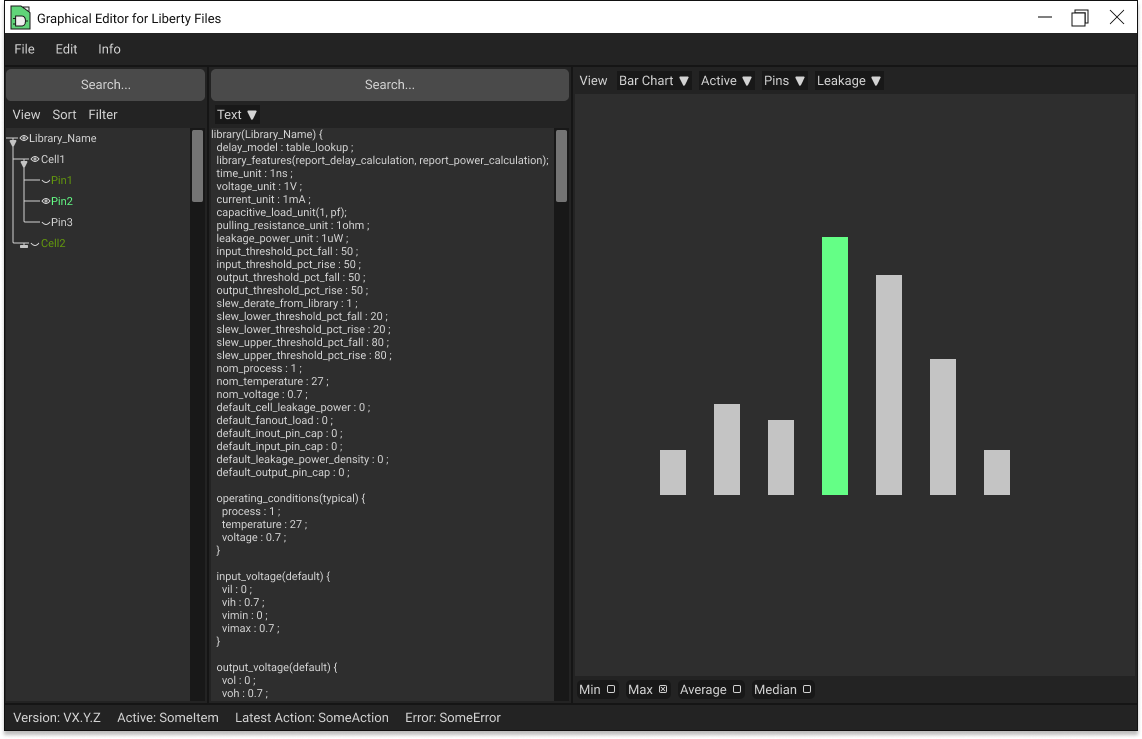
\includegraphics[scale=0.22]{Main Window}

\newpage
\section{Functional Requirements Overview}
\subsection{Mandatory Requirements List}
\begin{FR}
    \item \refer{FR-1}{Loading Liberty Files}
    \item \refer{FR-2}{Displaying Tree View of Liberty Files}
    \item \refer{FR-3}{Selecting elements}
    \item \refer{FR-4}{Opening an element in the working areas}
    % \item Navigating through elements in a display \label{FR-(-i)/67} % already described in the "Description" part of Displaying library/cell/pin
    \item \refer{FR-5}{Displaying a library}
    \item \refer{FR-6}{Displaying a cell}
    \item \refer{FR-7}{Displaying a pin}
    \item \refer{FR-8}{Visual comparison of attributes} % Can merge this one, because how displaying works has already been explained in Displaying a library/cell/pin. Merely describing how comparing works for different types of graphs should work.
    \item \refer{FR-9}{Searching for an element by name}
    \item \refer{FR-10}{Changing attributes through text editor}
    \item \refer{FR-11}{Searching in the text editor}
    \item \refer{FR-12}{Merging libraries}
    \item \refer{FR-13}{Resolving merge conflicts}
    \item \refer{FR-14}{Copying Cells into another Library}
    \item \refer{FR-15}{Removing a Library}
    \item \refer{FR-16}{Deleting Cells}
    \item \refer{FR-17}{Scaling graph values}
    \item \refer{FR-18}{Highlighting graph values}
    \item \refer{FR-19}{Viewing statistics for graphs}
    \item \refer{FR-20}{Saving a Liberty file}
    \item \refer{FR-21}{Saving a Library as a new File}
\end{FR}
\newpage 
\subsection{Optional Requirements List}
\begin{FRO}
    \item \refer{FRO-1}{Moving cells to another library}
    \item \refer{FRO-2}{Renaming elements}
    \item \refer{FRO-3}{Creating Liberty files from scratch}
    \item \refer{FRO-4}{Changing attributes through GUI}
    \item \refer{FRO-5}{Exporting data as CSV}
    \item \refer{FRO-6}{Resizing visualizer}
    \item \refer{FRO-7}{Popping visualizers out}
    \item \refer{FRO-8}{Re-positioning visualizers}
    \item \refer{FRO-9}{Saving a Liberty file into File Manager through drag-and-drop}
    \item \refer{FRO-10}{Saving all the Liberty files} 
    \item \refer{FRO-11}{Saving the state of a project}
    \item \refer{FRO-12}{Loading a project}
    \item \refer{FRO-13}{Exporting visualisations (graphs)}
    \item \refer{FRO-14}{Changing how the attributes of child elements are summarized}
    \item \refer{FRO-15}{Modifying the type of the graph}
    %\item Adding graph function visualisation through interpolation , 3D graphs scatter plot
    \item \refer{FRO-16}{Interpolating}
    % \item Applying formulas to graphs \label{FRO-12}
    % \item Magnifying the hitbox of a value on a histogram \label{FRO-13}
    \item \refer{FRO-17}{Changing GUI appearance}
    \item \refer{FRO-18}{Changing the preferences}
    \item \refer{FRO-19}{Changing the language}
    \item \refer{FRO-20}{Shortcuts}
    \item \refer{FRO-21}{Undo/Redo}
    \item \refer{FRO-22}{Viewing file properties}
    \item \refer{FRO-23}{Viewing application information} %has manual, github, version
    % \item Sorting \label{FRO-21}
    \item \refer{FRO-24}{Setting Filters for a search}
    \item \refer{FRO-25}{Setting default filters}
\end{FRO}
\newpage

\section{Functional Requirements}
\subsection{Mandatory Requirements}
\begin{FR}
    \item \FRDescription{Loading Liberty Files\label{FR-1}}
    {Ability to load, parse and create data objects from Liberty files with the desktop application}
    {Primary}
    {The selected files are in Liberty file format(not necessarily of the .lib extension), are not corrupted and fit into the memory}
    {The selected file(s) are:
    \begin{itemize}
        \item read
        \item parsed
        \item data objects based on the stored data are created
    \end{itemize}}
    {\begin{itemize}
        \item The selected file(s) are not loaded with the editor
        \item An appropriate IO error message is shown with the names of the problematic file(s) and a brief error description
    \end{itemize}}
    {\begin{itemize}
        \item Files are selected via File Manager (File >> Open)
        \item Files are dragged onto the desktop application and are dropped
    \end{itemize}}
    \item \FRDescription{Displaying Tree View of Liberty Files\label{FR-2}}
    {Ability to view the hierarchical structure of parsed Liberty files (from \ref{FR-1}) in a panel}
    {Primary}
    {\ref{FR-1} is performed successfully on the Liberty files to be viewed and the files fit into the memory}
    {The Liberty files from \ref{FR-1} can be viewed in Tree view in the said panel (Outliner).}
    {\begin{itemize}
        \item The hierarchical structure of the added Liberty files is not shown in the panel
        \item The added Liberty files are removed from the project
        \item What was shown in the panel before \ref{FR-2} remains unchanged
        \item An appropriate error message is shown
    \end{itemize}}
    {The successful execution of \ref{FR-1}}
    {\begin{itemize}
        \item Clicking on the collapse/expand component next to the name of the said parent element collapses/expands it's child elements
        \begin{itemize}
            \item If the said parent element is collapsed and the mentioned collapse/expand component is clicked, the said parent element is expanded.
            \item If the said parent element is expanded and the mentioned collapse/expand component is clicked, the said parent element is collapsed.
        \end{itemize}
    \end{itemize}}
    \item \FRDescription{Selecting elements\label{FR-3}}
    {Ability to select an element or multiple elements from the Tree View}
    {Primary}
    {Said element(s) is/are successfully loaded into the project}
    {Said element(s) is/are highlighted and selected}
    {An appropriate error message is shown}
    {\begin{itemize}
                \item Clicking on an element
                \item Clicking on multiple elements while holding CTRL key
            \end{itemize} }
    \item \FRDescription{Opening an element in the working area\label{FR-4}}
    {Ability to open an element in order to view or edit}
    {Primary}
    {Said element is successfully loaded into the project}
    {A visualizer is opened with:
    \begin{itemize}
        \item A close button 
        \item The tabs "Editor" and "View". The "View" tab is active by default, when the panel is created, where the "Editor" and "View" tabs are based on the open element.
    \end{itemize}}
    {An appropriate error message is shown}
    {\begin{itemize}
        \item A double click on an element
        \item Clicking on the Open component (Right-Click on the desired element >> Open)
    \end{itemize}}
    {\begin{itemize}
        \item When clicking on the "View" tab, the "View" panel is visible, and the "Editor" panel is minimised(not visible)
        \item When clicking on the "Editor" tab, the "Editor" panel is visible, and the "View" panel is minimised(not visible)
        \item When clicking the close button, the visualizer is closed and removed from the working area 
    \end{itemize}}
    \item \FRDescription{Displaying a Library\label{FR-5}}
    {Ability to view the values of attributes in a library}
    {Primary}
    {Said library is successfully loaded into the project}
    {On the View panel opened from \ref{FR-4} for a library
        \begin{itemize}
            \item The navigation view for Libraries is open
            \item A drop down list with the available attributes(input internal power,output internal power, leakage power, output timing)
            \item Drop down lists with the available (given in the liberty file) sub-attributes
            \begin{itemize}
                \item For internal power: power groups(fall-power, power and/or rise-power)
                \item For output timing: timing-sense (positive-unate, negative-unate and/or non-unate) timing-type(combinational, three-state-enable, etc.) and then timing groups (cell-fall, cell-rise, fall-transition, rise-transition, etc)
            \end{itemize}
            \item For the selected attribute (average values by default), a graph is drawn in the panel.
        \end{itemize}}
    {An appropriate error message is shown}
    {\begin{itemize}
        \item The "View" tab is made active
    \end{itemize}}
    {\begin{itemize}
        \item The navigation view for Libraries simply contains the cell names. Clicking on a cell name switches the visualizer to that of the corresponding cell that is shown through \ref{FR-6}
        \item Single value average default leakage power will be shown. According to the selected attribute, the following graph is drawn
        \begin{itemize}
            \item For the input internal power, a histogram with average input internal power is shown
            \item For the output internal power and output timing, a heatmap with the average will be shown
            \item For the leakage power, a bar chart is drawn with the averages of different input state powers (Like 000, 001, etc.)
                \begin{itemize}
                    \item In case a cell has 2 pins while another has 3, input state powers with 3 digits will be shown, but the leakage power will be taken by taking the last 2 digits into account for the 2 pin cells
                \end{itemize}
        \end{itemize}
    \end{itemize}}
    \item \FRDescription{Displaying a Cell\label{FR-6}}
    {Ability to view the values of attributes in a cell}
    {Primary}
    {Said cell is successfully loaded into the project}
    {On the View panel opened from \ref{FR-4} for a cell
    \begin{itemize}
        \item The navigation view for Cells is open
        \item A drop down list with the available attributes(input internal power,output internal power, leakage power, output timing)
        \item Drop down lists with the available (given in the liberty file) sub-attributes
            \begin{itemize}
                \item For internal power: power groups
                \item For output timing: timing-sense, timing-type and timing-group
            \end{itemize}
        \item For the selected attribute (average values by default), a graph is drawn in the panel.
    \end{itemize}}
    {An appropriate error message is shown}
    {\begin{itemize}
        \item The "View" tab is made active
    \end{itemize}}
    {\begin{itemize}
        \item The navigation view for a cell contains the visual representation of the cell. It has the correct number of drawn input/output pins and their names as well as checkboxes to the right of the input names. To the right of the output names is the output formula. Above the cell is the Library name
        \begin{itemize}
            \item Clicking on the Library name switches the visualizer to that of the parent library from \ref{FR-5}
            \item Clicking on an input/output pin switches the visualizer to that of the corresponding pin from \ref{FR-7}
            \item If the cell has more than 5 input pins or 3 output pins, the Visual representation gets changed with simple columns of input and output pins.
        \end{itemize}
        \item Single value default leakage power will be shown
        \item Single value leakage power will be shown calculated with the state of the active checkboxes close to the input pins alongside the formula. (When the checkbox is selected, current is flowing through it)
        According to the selected attribute, the following graph is drawn
        \begin{itemize}
            \item For the input internal power, a histogram with average input internal power is shown
            \item For the output internal power and output timing, a heatmap with the average will be shown
            \item For the leakage power, a bar chart is drawn with the different input state powers (Like 000, 001, etc.)
        \end{itemize}
    \end{itemize}}
    \item \FRDescription{Displaying a Pin\label{FR-7}}
    {Ability to view the values of attributes in a pin}
    {Primary}
    {Said pin is successfully loaded into the project}
    {On the View panel opened from \ref{FR-4} for a pin
        \begin{itemize}
            \item The navigation view for pins is open
            \item A drop down list with the available attributes(input internal power,output internal power, output timing)
            \begin{itemize}
                \item For input pins: internal power
                \item For output pins: internal power and timing
            \end{itemize}
            \item Drop down lists with the available (given in the liberty file) sub-attributes
            \begin{itemize}
                \item For internal power: power groups
                \item For timing: timing-sense, timing-type and timing groups
            \end{itemize}
            \item For the selected attribute, a graph is drawn in the panel.
        \end{itemize}}
    {An appropriate error message is shown}
    {\begin{itemize}
        \item The "View" tab is made active
    \end{itemize}}
    {\begin{itemize}
        \item The navigation view for a pin contains a visual representation of its parent cell with the highlighted current pin. It has the correct number of drawn input/output pins and their names as well as checkboxes(Only visible if current pin is output pin. Only one can be selected. First one is selected by default) to the right of the input names. To the right of the output names is the output formula. Above the cell is the Library name
        \begin{itemize}
            \item Clicking on the Library name switches the visualizer to that of the parent Library from \ref{FR-5}
            \item Clicking on the Cell itself switches the visualizer to that of the parent Cell from \ref{FR-6}
            \item Clicking on an input/output pin switches the visualizer to that of the corresponding pin from \ref{FR-7}
            \item If the cell has more than 5 input pins or 3 output pins, the visual representation gets changed with simple columns of input and output pins.
        \end{itemize}
        \item For output pins, function will be shown. 
        \item According to the selected attribute, the following graph is drawn
        \begin{itemize}
            \item For the input internal power, a histogram with average input internal power is shown
            \item For the output internal power and output timing, a heatmap with be shown according to the input pin whose checkbox is selected
        \end{itemize}
    \end{itemize}}
    \item \FRDescription{Visual comparison of attributes\label{FR-8}}
    {Compare the same type of attributes of different elements of the same type}
    {Primary}
    {The library, which contains the different elements, is successfully loaded into the project}
    {A comparison panel identical to the one in \ref{FR-4} except without the "Editor" subpanel is opened
        \begin{itemize}
            \item The selection view for the library or cells/pins is opened
            \item A drop down list with the available attributes(input internal power,output internal power, output timing, leakage power, default leakage power)
            \begin{itemize}
                \item For libraries: input/output internal power, timing, leakage power, default leakage power
                \item For cells: input/output internal power, timing, leakage power, default leakage power
                \item For input pins: internal power
                \item For output pins: internal power and timing
            \end{itemize}
            \item Drop down lists with the available (given in the liberty file) sub-attributes
            \begin{itemize}
                \item For internal power: power groups(fall-power, power and/or rise-power)
                \item For timing: timing-sense (positive-unate, negative-unate and/or non-unate) timing-type(combinational, three-state-enable, etc.) and then timing groups (cell-fall, cell-rise, fall-transition, rise-transition, etc)
            \end{itemize}
            \item For the selected attribute, a graph is drawn in the panel.
        \end{itemize}}
    {\begin{itemize}
        \item No new panel is opened
        \item An appropriate error message is shown
    \end{itemize}}
    {Clicking on Compare component (Right click after selecting multiple elements >> Compare).}
    {\begin{itemize}
        \item The selection view for a comparison of libraries contains a list of the selected libraries as well as checkboxes to their left (checkboxes filled by default).
        \begin{itemize}
            \item The libraries whose checkboxes are filled appear on the drawn graph
        \end{itemize}
        \item The selection view for a comparison of cells or pins shows the visual representation of all the cells involved like in the navigation bar as it appears in \ref{FR-7} for output pins
        \begin{itemize}
            \item By default, nothing is highlighted
            \item If the name of a cell, input pin or output pin is clicked, as long as no other element type is highlighted, it's highlighted and added to the graph.
            \item Like in \ref{FR-7} there are checkboxes on the left of the input pins that signify to which input pin the timing and internal power of the output pins are based on (The first one is selected by default)
        \end{itemize}
        \item According to the selected attribute, the following graph is drawn including only 2 elements
        \begin{itemize}
            \item For the input internal power, a histogram with the (average) input internal power is shown where histograms of different colors of are overlapping
            \item For the output internal power and output timing, a heatmap with the will be shown with the difference of the values being compared.
            \item For the leakage power, a bar chart is drawn with overlapping bars of different colors for the different input state powers (Like 001, 000, etc.)
            \begin{itemize}
                \item In case a cell has 2 pins while another has 3, input state powers with 3 digits will be shown, but the leakage power will be taken by taking the last 2 digits into account for the 2 pin cells
            \end{itemize}
        \end{itemize}
        \item If default average leakage power is selected, a bar chart is drawn comparing up to 10 elements.
    \end{itemize}}
    \item \FRDescription{Searching for an element by name\label{FR-9}}
    {Ability to search for an element by its name}
    {Primary}
    {There is an element with the given prefix}
    {The elements which contain the given prefix in their name are shown in the Outliner}
    {Nothing is shown in the Outliner}
    {Typing a string into the “search” textbox in the Outliner and pressing "Enter" key}
    \item \FRDescription{Changing attributes through text editor\label{FR-10}}
    {Ability to modify the loaded values of a library through the text editor in the "Editor" panel in the visualizer in the desktop application}
    {Primary}
    {Said library is successfully loaded into the project and has an visualizer opened through \ref{FR-4}}
    {\begin{itemize}
        \item Changes made in the text editor in the said "Editor" panel are reflected in the graphs and summaries.
        \item The corresponding library is modified.
    \end{itemize}}
    {\begin{itemize}
        \item Values in the library do not change
        \item The text editor in the said "Editor" panel goes back to its original value
        \item An appropriate error message is shown
    \end{itemize}}
    {Textually replacing the loaded values of a loaded Liberty file via the text editor in the said "Editor" panel.}
    \item \FRDescription{Searching in the text editor\label{FR-11}}
    {Ability to search for a given string in the text editor}
    {Primary}
    {\begin{itemize}
        \item The "Editor" panel of an element is opened
        \item The contents of the liberty file containing the element is being textually displayed in the text editor
    \end{itemize}}
    {\begin{itemize}
        \item The "Editor" scrolls to the point in text where the input string appears
        \item Every instance of the input string in the text is highlighted
    \end{itemize}}
    {An appropriate error message is shown}
    {Inputting a string in the search bar and pressing the "Enter" key}
    {Pressing the "Enter" key again scrolls the text to the next occurrence of the input string}
    \item \FRDescription{Merging libraries\label{FR-12}}
    {Ability to merge libraries into a new library}
    {Primary}
    {The initial libraries are successfully loaded into the project}
    {A new library will be created containing all the cells from the initial libraries}
    {\ref{FR-13} will be executed}
    {\begin{itemize}
        \item Clicking on Merge component (Right click after selecting the libraries >> Merge).
        % \item Clicking on Merge (Edit >> Merge) and then selecting the libraries to be merged
    \end{itemize}}
    \item \FRDescription{Resolving merge conflicts\label{FR-13}}
    {Ability to resolve merge conflicts caused by \ref{FR-12}}
    {Primary}
    {All involved libraries are successfully loaded into the project and they contain conflicting element names}
    {Conflict resolving pop outs will appear}
    {An appropriate error message is shown}
    {Executing \ref{FR-12} with conflicting files}
    {For every conflict a pop-up panel will appear which shows the occurring conflict. The resolving methods shown will be:
    \begin{itemize}
    \item Keeping either of the 2 cells by clicking the corresponding button
    \item Renaming either of the 2 cells in which case after typing the new name in the corresponding input box and then selecting the corresponding Rename button.
        \begin{itemize}
        \item In the case that the new name is also illegible, an error message will be shown alongside the prompt and the given name will be removed from the shown input box.
        \end{itemize}
    \item Aborting merge by clicking Close button. In which case the function from \ref{FR-12} will be cancelled and no new or existing liberty file will be changed.
\end{itemize}}
    \item \FRDescription{Copying cells into another library\label{FR-14}}
    {Ability to copy cells into a library}
    {Primary} 
    {All involved libraries are successfully loaded into the project}
    {The copied cells from the original libraries are pasted into the destination library}
    {The same conflict resolution from \ref{FR-13} takes place with minor differences.
    \begin{itemize}
        \item Instead of creating a new library, the destination library is modified
        \item In case the Close button is clicked, neither of the libraries in question is modified
    \end{itemize}}
    {\begin{itemize}
        \item Selecting a/multiple cell(s) and pressing CTRL+C followed by selecting another element and pressing CTRL+V
        \item Clicking on the Copy component (Right-Click on the desired cell >> Copy) followed by clicking on the paste component (Right-Click on the desired element >> Paste)
    \end{itemize}}
    \item \FRDescription{Removing a library\label{FR-15}}
    {Ability to remove a library from the project}
    {Primary}
    {Said library is successfully loaded into the project}
    {The opened library is removed from the project and the Outliner}
    {\begin{itemize}
        \item No library is modified
        \item An appropriate error message is shown
    \end{itemize}}
    {\begin{itemize}
        \item Clicking on the "Remove" component (Right-Click on the desired library >> Remove)
        \item Selecting multiple libraries and clicking on the "Remove" component (Right-Click on one of the selected libraries  >> Remove)
    \end{itemize}}
    \item \FRDescription{Deleting cells\label{FR-16}}
    {Ability to delete a/multiple cell(s) from a library}
    {Primary}
    {The library, which contains the mentioned cell(s), is successfully loaded into the project}
    {The mentioned cell(s) is/are deleted from their library and removed from the Outliner}
    {\begin{itemize}
        \item No library is modified (no cell(s) is/are removed)
        \item An appropriate error message is shown
    \end{itemize}}
    {\begin{itemize}
        \item Clicking on the "Delete" component (Right-Click on the desired Cell  >> Delete)
        \item Selecting multiple cells and clicking on the "Delete" component (Right-Click on one of the selected cells  >> Delete)
    \end{itemize}}
    \item \FRDescription{Scaling graph values\label{FR-17}}
    {Scaling the values of a graph by a given factor}
    {Primary}
    {\ref{FR-5},\ref{FR-6} or \ref{FR-7} is performed on the element, which contains the above mentioned values}
    {The mentioned values are scaled by the given factor and changes are reflected in the loaded element.}
    {\begin{itemize}
        \item No value will be changed
        \item An appropriate error indicator will be shown. %Examples:
        %\begin{itemize}
            %\item If the factor is to be written in a textbox and no buttons are involved:
            %\begin{itemize}
            %    \item Highlighting the given factor
            %    \item Displaying an “invalid value” text next to the textbox, in which the given factor is written
            %\end{itemize}
            %\item If there are buttons or dedicated windows are involved:
            %\begin{itemize}
            %    \item An appropriate error message will be shown
            %\end{itemize}
        %\end{itemize}
    \end{itemize}}
    {Clicking on "Scale by value" Component (Right-Click on said graph >> Scale by value). Then entering the desired value on the input box and clicking "Confirm"}
    \item \FRDescription{Highlighting graph values\label{FR-18}}
    {Ability to highlight a certain value from a graph}
    {Primary}
    {\ref{FR-4} is executed on a given element successfully}
    {The source of the said value and the value itself is highlighted}
    {An appropriate error message is shown}
    {Hovering the mouse pointer over the said value in it's graph}
    {\begin{itemize}
        \item The element, which contains the mentioned value, and it's parent elements are highlighted in the tree view.
        \item If the visualizer of the said element has the "Editor" tab active as well, the value itself in the text editor in the "Editor" tab will be highlighted.
    \end{itemize}}
    \item \FRDescription{Viewing statistics for graphs\label{FR-19}}
    {Ability to view the desired statistics of the values of an attribute in a graph}
    {Primary}
    {\ref{FR-5},\ref{FR-6} or \ref{FR-7} is executed on a given element successfully}
    {The desired statistics of the said attributes are shown in the graph with:
    \begin{itemize}
        \item Horizontal line(s) (y = value of the desired statistic, in a cartesian coordinate system), if the said graph is a histogram or we need the average value in a bar chart or median in a bar chart with even entries.
        \item Re-colouring the values that are similar (or are) the values of the desired statistics, if the said graph is a heatmap.
        \item Highlighting the bar that fulfills the desired statistic in a bar chart.
    \end{itemize}}
    {\begin{itemize}
        \item No statistics are shown
        \begin{itemize}
            \item If other statistics were already being shown, they remain unchanged
        \end{itemize}
        \item An appropriate error message is shown
    \end{itemize}}
    {Clicking on the checkboxes below the graph.}
    {\begin{itemize}
        %%% I don't get this -Xhulio %%% \item (?) The similarity mentioned in the "Post Condition (success)" part can be modified via it's dedicated component (?)
        \item The available statistics are Min(minimum), Max(maximum), Average and Median.
        \item The way of showing statistics in graphs mentioned in the "Post Condition (success)" and the graphs use different colours to make it easier for the user to distinguish them from each other.
        \item In comparison graphs, only one unique statistic appears for the entire graph.
    \end{itemize}}
    \item \FRDescription{Saving a Liberty file\label{FR-20}}
    {Ability to save changes made to a Liberty file}
    {Primary}
    {Corresponding library is successfully loaded into the project}
    {Said Liberty file is modified corresponding to the version in the project}
    {\begin{itemize}
        \item No Liberty file is modified
        \item An appropriate error message is shown
    \end{itemize}}
    {Clicking on the Save component (Right-Click on the desired Library  >> Save)}
    \item \FRDescription{Saving a library as a new file\label{FR-21}}
    {Ability to save a library as a new Liberty file}
    {Primary}
    {Said library is successfully loaded into the project}
    {A new liberty file is created corresponding to the version in the project}
    {\begin{itemize}
        \item No new liberty file is created
        \item An appropriate error message is shown
    \end{itemize}}
    {Clicking on the Save As component (Right-Click on the desired Library  >> Save As)}
    {\begin{itemize}
        \item The corresponding base liberty file (if present) will not be changed throughout the entire process.
    \end{itemize}}
\end{FR}

\subsection{Optional Requirements}

\begin{FRO}
    \item \FRODescription{Moving cells to another library\label{FRO-1}}
    {Ability to move a/multiple cell(s) to a library}
    {Optional}
    {All involved libraries are successfully loaded into the project}
    {\begin{itemize}
        \item The mentioned cell(s) from the original libraries are moved to the destination library
        \item The mentioned cell(s) are deleted from the origin library
    \end{itemize}}
    {The same conflict resolution from \ref{FR-13} takes place with the minor adjustments further explained in the Post Condition (fail) from \ref{FR-14}}
    {Drag-dropping the cell(s) within the Outliner, from it's own library into another library}
    \item \FRODescription{Renaming elements\label{FRO-2}}
    {Ability to rename elements in a loaded library}
    {Optional}
    {The new name of the component is not conflicting with the name of one of the existing ones within the same library}
    {The mentioned element is renamed to their desired new name}
    {\begin{itemize}
        \item The current name of the component to be renamed is unchanged
        \item An appropriate error message is shown
    \end{itemize}}
    {Clicking on the "Rename" component (Right-Click on the desired Element  >> Rename)}
    \item \FRODescription{Creating Liberty files from scratch\label{FRO-3}}
    {Ability to create a new liberty file via the text editor}
    {Optional}
    {The input in the said text editor is valid and in liberty file format}
    {The input in the said text editor is opened into the project as a new library}
    {\begin{itemize}
        \item The current input in the text editor of the GUI of the desktop application is unchanged.
        \item An appropriate error message is shown
    \end{itemize}}
    {\begin{itemize}
        \item Clicking on the “New” component (File >> New) to open the text editor
        \item Clicking on the "Save" component (Top right screen of the opened editor) to save the input in the said text editor as a new liberty file.
    \end{itemize}}
    {\begin{itemize}
    \item The text editor looks like the normal editor opened in the visualizers from \ref{FR-4} except:
        \begin{itemize}
            \item It has no "View" panel.
            \item It doesn't dynamically update.
            \item It has a Save button on the top right corner.
        \end{itemize}
    \item The inputted library is automatically opened in the project
    \end{itemize}}
    \item \FRODescription{Changing attributes through GUI\label{FRO-4}}
    {Ability to modify the values of an element from it's value occurrence in the "View" panel}
    {Optional}
    {\ref{FR-5}, \ref{FR-6} or \ref{FR-7} is successfully performed on said element}
    {\begin{itemize}
        \item Changes made in the "View" panel are reflected in the graphs and summaries.
        \item The corresponding library is modified.
    \end{itemize}}
    {\begin{itemize}
        \item Values in the library don’t change
        \item Values in the "View" panel don't change
        \item An appropriate error message is shown
    \end{itemize}}
    {Double-clicking on a value, inserting a new value in the input box and then pressing the "Enter" Key}
    {Said value can be a single value printed in the "View Panel or part of a drawn graph}
    \item \FRODescription{Exporting data as CSV\label{FRO-5}}
    {Ability to export the data of a given element in Comma-Separated Values (CSV) format}
    {Optional}
    {Said element is successfully loaded into the project}
    {The data within the said element has been exported as a new file in CSV format}
    {\begin{itemize}
        \item No new files are made
        \item An appropriate error message is shown
    \end{itemize}}
    {Clicking on the “Export as CSV” component (Right-click on the desired element >> Export as CSV) and choosing the desired path through the File Manager.}
    \item \FRODescription{Resizing visualizers\label{FRO-6}}
    {Ability to resize an visualizer opened}
    {Optional}
    {Said visualizer is successfully opened through \ref{FR-4}}
    {The visualizers have different sizes}
    {\begin{itemize}
        \item No visualizers are changed
        \item An appropriate error message is shown
    \end{itemize}}
    {Clicking on on the border between two visualizers and adjusting it to modify their sizes}
        \item \FRODescription{Popping elements panels out\label{FRO-7}}
    {Ability to pop out an visualizer as a new window}
    {Optional}
    {\begin{itemize}
        \item Said visualizer is successfully opened through \ref{FR-4}
        \item Said element is loaded into the project and 3 (three) visualizers are already open.
    \end{itemize}}
    {The visualizer is opened as a new window}
    {\begin{itemize}
        \item No visualizers are changed
        \item An appropriate error message is shown
    \end{itemize}}
    {\begin{itemize}
        \item Clicking on an visualizers title and dragging it outside of the working area area
        \item Trying to open a new visualizer through \ref{FR-4} once 3 (three) visualizers are already opened in the working area
    \end{itemize}}
    {Popped out visualizers can be returned to the working area by dragging them and dropping them in the working area} %?????????? THIS DECIDES HOW THE TITLE SHOULD LOOK LIKE
    \item \FRODescription{Re-positioning visualizers\label{FRO-8}}
    {Ability to change the order of the visualizers in the working area}
    {Optional}
    {At least 2(two) visualizers are successfully opened through \ref{FR-4}}
    {The visualizers have the new specified positions}
    {\begin{itemize}
        \item No visualizers have switched positions
        \item An appropriate error message is shown
    \end{itemize}}
    {Clicking on an visualizers title and dragging it to the new position desired within the working area}
    {visualizers shift to the left or right so that the dropped visualizer is placed on the position it was dropped}
    \item \FRODescription{Saving a liberty file into File Manager through drag-drop\label{FRO-9}}
    {Ability to save a loaded liberty file into File Manager by using drag-drop}
    {Optional}
    {Said library is successfully loaded into the project}
    {The mentioned liberty file is saved at the given path}
    {\begin{itemize}
        \item The current status of the loaded liberty file is unchanged
        \item No new files are created
        \item An appropriate error message is shown
    \end{itemize}}
    {Selecting a/multiple loaded Liberty file(s) in the Tree view and dragging it/them to the desired location in the File Manager}
    \item \FRDescription{Saving all the Liberty files\label{FRO-10}}
    {Ability to save changes made to all Liberty file}
    {Optional}
    {None}
    {\begin{itemize}
        \item All Liberty files loaded through \ref{FR-1} are modified corresponding to the version in the working area
        \item A pop up window reminds the user of the libraries not yet assigned a path where they can be saved as Liberty files
    \end{itemize}}
    {\begin{itemize}
        \item No Liberty file is modified
        \item An appropriate error message is shown
    \end{itemize}}
    {Clicking on the "Save all" component (Right-Click on the desired Library  >> Save all)}
    \item \FRODescription{Saving the state of a project\label{FRO-11}}
    {Ability to store the state of a project for future use}
    {Optional}
    {At least one library is successfully loaded into the project}
    {The current status of the project will be saved in a JSON file}
    {\begin{itemize}
        \item The project remains unchanged
        \item An appropriate error message is shown
    \end{itemize}}
    {Clicking on the designated “Save Project” component (File >> Save Project)}
    \item \FRODescription{Loading a project\label{FRO-12}}
    {Ability to re-use a (valid) past project}
    {Optional}
    {The selected project save file (created from \ref{FRO-11}) has the right format, is not corrupted and fits into the memory}
    {The chosen past project is loaded}
    {\begin{itemize}
        \item The current project is unchanged
        \item An appropriate error message is shown
    \end{itemize}}
    {Clicking on the designated “Open Project” component (File >> Open Project) and selecting said project file through the File Manager}
    {Fully replaces the current project. 
    \begin{itemize}
    \item If the current project is not empty, a pop-up window will show to confirm the action. 
    \item In case one of the liberty files is not found on the specified path, a pop-up panel notifies the error and the said file does not show up in the hierarchical structure or open in the working area
    \end{itemize}}
    \item \FRODescription{Exporting visualisations (graphs)\label{FRO-13}}
    {Ability to store created graphs for future use}
    {Optional}
    {The said graph has been created successfully through \ref{FR-5}, \ref{FR-6} or \ref{FR-7}}
    {The mentioned graph is saved as an image file}
    {\begin{itemize}
        \item No new files are created
        \item An appropriate error message is shown
    \end{itemize}}
    {Clicking on the designated “Export Graph” component (Right-click on said graph >> Export Graph) and then selecting where to save the image and in what format through the File Manager}
    \item \FRODescription{Changing how the attributes of child elements are summarised\label{FRO-14}}
    {Ability to change a graphs data to represent minimum, maximum or average values if possible}
    {Optional}
    {\ref{FR-5}, \ref{FR-6} or \ref{FR-7} has been successfully performed on the given element and the desired attribute has minimum and maximum values specified}
    {The current graph is replaced by one with the desired data}
    {\begin{itemize}
        \item The current graph is unchanged
        \item An appropriate error message is shown
    \end{itemize}}
    {Clicking on the dropdown box component and selecting the type of summary}
    \item \FRODescription{Modifying the type of the graph\label{FRO-15}}
    {Making viewing the values of desired attributes of desired elements in different graph types possible}
    {Optional}
    {\ref{FR-5}, \ref{FR-6},\ref{FR-7} or \ref{FR-8} is performed on an element or multiple elements successfully}
    {The type of the graph changes to the desired graph type}
    {\begin{itemize}
        \item The graph is unchanged
        \item An appropriate error message is shown
    \end{itemize}}
    {Clicking on the corresponding drop down component in the "View" panel of the visualizer and choosing the new type of the graph}
    {The graph types to be added are:
    \begin{itemize}
        \item Scatterplot that would work in every instance of Histograms. in Histogram comparisons, the values would have different colors according to the corresponding element.
        \item Function graph that would work in every instance of Histograms by interpolating the values. In comparison, graphs would be overlaid with different colors.
        \item 3D graphs that would work in every instance of heatmaps. In comparisons it would represent the difference between the values being compared.
        \item Tabular view (simple data table) that would work in every instance of heatmaps. In comparisons, it would just show both values and their difference
    \end{itemize}}
    \item \FRODescription{Interpolating\label{FRO-16}}
    {Calculating approximations for the values of indexes that aren't given in the Liberty File}
    {Optional}
    {\ref{FR-5}, \ref{FR-6} or \ref{FR-7} is performed on an element successfully}
    {The value is shown in the text box}
    {An appropriate error message is shown}
    {Clicking on the corresponding "Interpolate" Component on the bottom right of the graph, inserting a value (or two) and pressing "Enter" key}
    {The opened window when pressing the Interpolate component has an input (or two) box, a text box where the final value is shown and a "Close" button}
    %Decided as unnecessary
%    \item \FRODescription{Applying formulas to graphs}
%    {Using a given mathematical expression (such as a function) on the values shown in a graph}
%    {Optional}
%    {\begin{itemize}
%        \item The said graph has been created successfully with \ref{FR-3}
%        \item The given mathematical expression is valid (semantically and syntactically)
%    \end{itemize}}
%    {The mentioned mathematical expression is used on the values shown in the selected graph and the %      graph is updated.}
%    {\begin{itemize}
%        \item Mentioned values are unchanged
%        \item Mentioned graph is unchanged
%        \item An appropriate error message is shown (for example in the input bar)
%    \end{itemize}}
%    {Typing a mathematical expression as a string in the “input bar” component}
    % Decided as unnecessary
%    \item \FRODescription{Magnifying the hitbox of a value on a histogram}
%    {Ability to make the hitbox of a value on a graph bigger}
%    {Optional}
%    {\ref{FR-3} is performed on an attribute of a Liberty file successfully}
%    {The desired value in the graph gets a larger hitbox}
%    {\begin{itemize}
%        \item The histogram is unchanged
%        \item An appropriate error message is shown
%    \end{itemize}}
%    {Left clicking on a value in a histogram}
    \item \FRODescription{Changing GUI appearance\label{FRO-17}}
    {Ability to customise the appearance of the GUI}
    {Optional}
    {None}
    {The desired GUI appearance has been changed.}
    {\begin{itemize}
        \item Appearance remains unchanged
        \item An appropriate error message is shown
    \end{itemize}}
    {Appearance can be changed under the “Appearance” panel (Edit panel >> Settings >> Appearance) . Then changing the desired appearance element}
    {\begin{itemize}
        \item Change graph default type, their color or the color/ size/ type of their fonts
        \item Changing the overall theme/ background color
        \item Scaling the font size
    \end{itemize}}
    \item \FRODescription{Changing the preferences\label{FRO-18}}
    {Ability to customise the functionality of the desktop application}
    {Optional}
    {None}
    {The functionalities of the desktop application changes to the desired one}
    {\begin{itemize}
        \item The past functionality of the desktop application is unchanged
        \item An appropriate error message is shown
    \end{itemize}}
    {Preferences can be changed under the “Preferences” panel (Edit panel >> Settings >> Preferences) . Then changing the desired preferences}
    {\begin{itemize}
        \item Set the number of undo/redo operations the application should try to support
        \item Set the maximum number of bars able to be displayed in a bar chart
        \item Set the default subpanel opened when a new visualizer is opened (Editor or View)
    \end{itemize}}
    \item \FRODescription{Changing the language\label{FRO-19}}
    {Ability to change the default language of the desktop application}
    {Optional}
    {The files regarding the new language exist and can be located by the desktop application}
    {The current language will be replaced with the desired one}
    {An appropriate error message is shown}
    {Clicking on the “Change language” component (Edit panel >> Settings >> Preferences >> Change Language) . Then selecting the desired language}
    \item \FRODescription{Shortcuts\label{FRO-20}}
    {Ability to access the functionality faster}
    {Optional}
    {\begin{itemize}
        \item The shortcut is performed correctly by the user
        \item The corresponding functionality can be used in the current state of the project
    \end{itemize}}
    {The corresponding functionality is executed without their triggering component}
    {\begin{itemize}
        \item The state of the project is unchanged
        \item An appropriate error message is shown
    \end{itemize}}
    {Pressing the shortcut keys}
    {Shortcuts can be changed under the “Shortcuts” panel (Edit panel >> Settings >> Shortcuts) . Then setting the desired keys for the set events}
    \item \FRODescription{Undo/Redo\label{FRO-21}}
    {Ability to move backward (Undo)/forward (Redo) in the history of the project}
    {Optional}
    {There are actions done, which can be undone/redone}
    {The desired state of the project is set as the current state}
    {\begin{itemize}
        \item The current state of the project is unchanged
        \item The undo/redo component is disabled
    \end{itemize}}
    {Clicking on the “undo”/”redo” component}
    {The maximum amount of actions a user can undo at a given time is 10 by default (if \ref{FRO-18} is not implemented).}
    \item \FRODescription{Viewing file properties\label{FRO-22}}
    {Ability to view the properties of a liberty file, such as: file location, file size}
    {Optional}
    {Corresponding library is successfully loaded into the project}
    {A window with the properties of the loaded liberty file is shown}
    {An appropriate error message is shown}
    {Clicking on the "Properties" component (Right-Click on the corresponding library  >> Properties)}
    \item \FRODescription{Viewing application information\label{FRO-23}}
    {Ability to view the information related to the desktop application}
    {Optional}
    {None}
    {Corresponding information is shown as detailed in the description}
    {An appropriate error message is shown}
    {Clicking on the desired information (Info panel >> Manual/Github/About)}
    {\begin{itemize}
        \item Manual opens a document containing instructions to the applications functionality
        \item Github activates a hyperlink to the applications github website
        \item About opens a window with general information about the application
        \item General information about app version, selected elements and/or latest operation is displayed in the Info bar 
    \end{itemize}}
    % Decided as unnecessary last time?
%    \item \FRODescription{Sorting}
%    {Ability to sort the shown information in order to make viewing easier}
%    {Optional}
%    {None}
%    {The desired piece of shown information in the Outliner is sorted}
%    {An appropriate error message is shown}
%   {Clicking on the “Sort by” component and selecting how and what to sort after (i.e.: name, value, % %   ascending, descending) using the designated component}
    \item \FRODescription{Setting Filters for a search\label{FRO-24}}
    {Ability to add/remove a filter of an element for its attribute values or lack thereof}
    {Optional}
    {None}
    {Filter is added or removed as a search filter}
    {\begin{itemize}
        \item An appropriate error indicator will be shown. Examples:
        \begin{itemize}
            \item Invalid attribute name
            \item Invalid value
        \end{itemize}
        \item Attribute filters for the search bar remain unchanged
    \end{itemize}}
    {Modifying filters components in the “Filter” component}
    {Upon clicking the “Filter” component a new pop-up panel opens up that shows all active filters. There filters can be removed by clicking the “Remove“ component next to the filter. Filters can be added by selecting attribute name, filter type, adding filter value and then clicking the “Add Filter” component}
    \item \FRODescription{Setting default attribute filters\label{FRO-25}}
    {Saving a given set of attribute filters as the default filter}
    {Optional}
    {At least 1 filter added through \ref{FRO-24} is active}
    {The mentioned set of attribute filters are set as the default filter for whenever the application is run anew.}
    {\begin{itemize}
        \item The past default filter is still the default filter
        \item An appropriate error message is shown
    \end{itemize}}
    {Clicking on the “Set as default filter” component in the Filter component from \ref{FRO-24}}
\end{FRO}

\section{Non-Functional Requirements}
\subsection{Core}
\subsubsection{Reliability}
\begin{NFR-Rel}
    \item The desktop application should be able to open at least 2 liberty files at the same time
    \item At least 10 drawn graphs should be able to exist
    \item The desktop application should be able to handle liberty files with a size of up to [Example file *10] MB
\end{NFR-Rel}

\subsubsection{Performance}
\begin{NFR-Perf}
    \item A liberty file should take no longer than 1 second to load
    \item A graph should be drawn in no longer than 5 seconds
    \item The desktop application should not be able to run twice at the same time
    \item  The desktop application should not be able to support more than 3 visualizers in the working area
\end{NFR-Perf}

\subsection{Robustness}
\begin{NFR-Rob}
    \item Taking different library units into account
\end{NFR-Rob}

\subsection{Optional}
\subsubsection{Usability}
\begin{NFRO-Usability}
    \item The desktop application should be able to support English, German, French, Albanian and Turkish
    \item The desktop application should be able to restore at least the 5 previous states for the undo/redo operations 
\end{NFRO-Usability}

\subsubsection{Performance}
\begin{NFRO-Perf}
    \item A Liberty file should take no longer than 20 milliseconds to load
    \item A graph should be drawn in no longer than 1 second
\end{NFRO-Perf}

\chapter{Global Test Cases}

\section{Global test cases for functional requirements}


\begin{GTC}
    \item \refer{GTC-1}{(tests FR-1 and FR-2) Successfully open a Liberty file}
    \item \refer{GTC-2} {(tests FR-1 and FR-2) Successfully open multiple Liberty files}
    \item \refer{GTC-3} {(tests FR-1) Failed loading of a file}
    \item \refer{GTC-4} {(tests FR-3) Select an element}
    \item \refer{GTC-5} {(tests FR-3) Select multiple elements}
    \item \refer{GTC-6} {(tests FR-3) Collapse and expand elements}
    \item \refer{GTC-7} {(tests FR-4, FR-5) Open the library in the working panel}
    \item \refer{GTC-8} {(test FR-5) Display a histogram for average internal power of input pins of the selected library}
    \item \refer{GTC-9} {(tests FR-5) Display a heat map for internal power or timing of output pins of the selected library}
    \item \refer{GTC-10} {(tests FR-5) Display a bar chart for the power leakage values of cells with same number of input pins}
    \item \refer{GTC-11} {(tests FR-5) Display a bar chart for the power leakage values of cells with different number of input pins}
    \item \refer{GTC-12} {(tests FR-5) Click on a cell name on the library view to go that cell's view}
    \item \refer{GTC-13} {(tests FR-6) Display a cell with an image}
    \item \refer{GTC-14} {(tests FR-6) Display a cell with too many inputs}
    \item \refer{GTC-15} {(tests FR-6, FR-5) Click the library name to go from the cell view to library view}
    \item \refer{GTC-16} {(tests FR-6) Select checkboxes of input pins to determine the function of the cell}
    \item \refer{GTC-17} {(tests FR-6) Display leakage value of a cell with a bar chart}
    \item \refer{GTC-18} {(tests FR-6, FR-7) Click on the name of a pin to go from the cell view to pin view}
    \item \refer{GTC-19} {(tests FR-7) Display a pin}
    \item \refer{GTC-20} {(tests FR-7) Display timing or internal power of output pins with a heat map}
    \item \refer{GTC-21} {(tests FR-7) Display internal power for input pins with a histogram}
    \item \refer{GTC-22} {(tests FR-7) Click on the name of the cell the pin belongs to in order to go from pin view to cell view}
    \item  \refer{GTC-23} {(tests FR-8) Compare input pins with each other}
    \item  \refer{GTC-24} {(tests FR-8) Compare output pins with each other}
    \item  \refer{GTC-25} {(tests FR-8) Compare cells with each other}
    \item  \refer{GTC-26} {(tests FR-8) Compare libraries with each other}
    \item  \refer{GTC-27} {(tests FR-9) Merging two libraries}
    \item  \refer{GTC-28} {(tests FR-9 and FR-10) Resolve a merge conflict by renaming}
     \item  \refer{GTC-29} {(tests FR-9 and FR-10) Resolve a merge conflict by keeping one cell}
    \item  \refer{GTC-30} {(tests FR-9 and FR-10) Aborting merge conflict}
    \item  \refer{GTC-31} {(tests FR-11) Copying a cell into another library which does not have a cell with the same name}
    \item  \refer{GTC-32} {(tests FR-11) Copying multiple cells into another library which does not have a cell with the same name}
    \item  \refer{GTC-33} {(tests FR-11) Copying a cell into another library where a cell with the same name exists.}
    \item  \refer{GTC-34} {(tests FR-12) Removing a library}
    \item  \refer{GTC-35} {(tests FR-12) Removing multiple libraries}
    \item  \refer{GTC-36} {(tests FR-13) Deleting a cell from a library}
    \item  \refer{GTC-37} {(tests FR-14) Searching for an attribute in the text editor}
    \item  \refer{GTC-38} {(tests FR-15) Editing a cells default leakage power through text editor panel}
    \item  \refer{GTC-39} {(tests FR-15) Editing a cells default leakage power through text editor with an invalid value}
    \item  \refer{GTC-40} {(tests FR-16) Scaling with a valid value}
    \item  \refer{GTC-41} {(tests FR-16) Scaling with an invalid value}
    \item  \refer{GTC-42} {(tests FR-17) Highlighting an attribute of a cell through a graph}
    \item  \refer{GTC-43} {(tests FR-18)  Displaying minimum value for input internal power on a histogram}
    \item  \refer{GTC-44} {(tests FR-18)  Displaying maximum value for output internal power on the heat map}
    \item  \refer{GTC-45} {(tests FR-18)  Displaying the average and median values for leakage powers on a graph}
    \item  \refer{GTC-46} {(tests FR-19) Searching for a cell}
    \item  \refer{GTC-47} {(tests FR-19) Searching for a cell that does not exist in the loaded library}
    \item  \refer{GTC-48} {(tests FR-20) Saving changes in a library}
    \item  \refer{GTC-49} {(tests FR-21) Saving a library as a new file}
    
\end{GTC}

\section{Global test cases for optional requirements}
\begin{GTCO}
    \item  \refer{GTCO-1}{(tests FRO-1) Move a cell to another library}
    \item  \refer{GTCO-2}{(tests FRO-2) Rename an element}
    \item  \refer{GTCO-3}{(tests FRO-3) Create a liberty file}
    \item  \refer{GTCO-4}{(tests FRO-4) Change attributes from the UI}
    \item  \refer{GTCO-5}{(tests FRO-5) Export data as CSV}
    \item  \refer{GTCO-6}{(tests FRO-6) Resize an visualizer}
    \item  \refer{GTCO-7}{(tests FRO-7) Pop out the panel of an element}
    \item  \refer{GTCO-8}{(tests FRO-8) Switch positions of visualizers}
    \item  \refer{GTCO-9}{(tests FRO-9) Save a Liberty File using drag-drop}
    \item  \refer{GTCO-10}{(tests FRO-10) Save all Liberty files at the same time}
    \item  \refer{GTCO-11}{(tests FRO-11) Save the current state of a project}
    \item  \refer{GTCO-12}{(tests FRO-12) Load a project}
    \item  \refer{GTCO-13}{(tests FRO-13) Export a graph}
    \item  \refer{GTCO-14}{(tests FRO-14) Showing only minimum and maximum input internal power of a pin}
    \item  \refer{GTCO-15}{(tests FRO-15) Changing the heat map of a pin’s timing values to a 3D graph}
    \item  \refer{GTCO-16}{(tests FRO-15) Changing the bar chart of leakage power values to a scatterplot}
    \item  \refer{GTCO-17}{(tests FRO-16) Interpolating a histogram}
    \item  \refer{GTCO-18}{(tests FRO-17)  Changing chart’s colour}
    \item  \refer{GTCO-19}{(tests FRO-17) Changing font size of an attribute on a chart}
    \item  \refer{GTCO-20}{(tests FRO-18) Changing default chart colour }
    \item  \refer{GTCO-21}{(tests FRO-18) Changing the default font size}
    \item  \refer{GTCO-22}{(tests FRO-19) Changing GUI display colour}
    \item  \refer{GTCO-23}{(tests FRO-20) Changing the language to German}
    \item  \refer{GTCO-24}{(tests FRO-21) Using a shortcut}
    \item  \refer{GTCO-25}{(tests FRO-22) Undoing a change}
    \item  \refer{GTCO-26}{(tests FRO-22) Reverting an undo}
    \item  \refer{GTCO-27}{(tests FRO-23) Viewing the properties of the library baseline.lib}
    \item  \refer{GTCO-28}{(tests FRO-24) Viewing app information}
    \item  \refer{GTCO-29}{(tests FRO-25) Setting a value filter for an attribute.}
    \item  \refer{GTCO-30}{(tests FRO-26) Setting a default attribute filter}
    
\end{GTCO}

\section{Test cases}

 % baseline.lib and different1.lib are Liberty files that were provided, which are used in the following tests to evaluate the functionality. 
  
\begin{GTC}
    \item \GTCDescription{\ref{FR-1} and \ref{FR-2}}
    {Successfully open a Liberty File} \leavevmode \\ 
        \action{User selects "Open" in the menu and selects a Liberty File from the File Manager.}
        \reaction{Selected Liberty File is displayed hierarchically in a tree view on the left side (Outliner) of the desktop app.} \label{GTC-1}
        
    \item \GTCDescription{\ref{FR-1} and \ref{FR-2}}
    {Successfully open multiple Liberty Files} \leavevmode \\ 
        \action{User selects "Open" in the menu to select two Liberty Files.}
        \reaction{Both liberty files are displayed hierarchically in a tree view on the left side (Outliner) of the desktop app.}\label{GTC-2}
        
    \item \GTCDescription{\ref{FR-1}}
    {Failed loading of a file} \leavevmode \\ 
        \precondition{Selected file is not on liberty format.}
        \action{User selects "Open" in the menu and selects said file.}
        \reaction{No file is displayed on the app. A file not found error is displayed.}\label{GTC-3}
        
    \item \GTCDescription{\ref{FR-3}}
    {Select an element} \leavevmode \\ 
        \precondition{At least one Liberty File is opened in the app and the file has at least one element.}
        \action{User clicks on the desired element.}
        \reaction{The element is highlighted.}\label{GTC-4}
        
    \item \GTCDescription{\ref{FR-3}}
    {Select multiple elements} \leavevmode \\ 
        \precondition{At least one Liberty File is opened in the app and the file has at least two elements.}
        \action{User holds CTRL and clicks multiple elements.}
        \reaction{Clicked elements are highlighted.}\label{GTC-5}
        
        
    \item \GTCDescription{\ref{FR-2}}
    {Collapse and expand elements} \leavevmode \\ 
        \precondition{Elements expanded or collapsed have child elements.}
        \state{Liberty file is opened and it's tree view is displayed on the left.}
        \action{User clicks on collapse button next to the element (Library or Cell).}
        \reaction{Child elements are hidden. Cells are hidden for the selected library and pins are hidden for a selected cell.}
        \action{User clicks on expand button next to the element (Library or Cell).}
        \reaction{Child elements are visible again. Cells of the selected library are visible and pins are visible for the selected cell.}\label{GTC-6}
    
    \item \GTCDescription{\ref{FR-4} and \ref{FR-5}}
    {Open the library in the working panel} \leavevmode \\ 
        \precondition{At least one Liberty File is opened in the app.}
        \state{Tree view of the Liberty file is displayed on the left.}
        \action{User right clicks the library in the tree view and clicks "Open".}
        \reaction{The selected library is opened in a new panel.}
        \state{The new panel has the options "Editor" and "View" ."View" is opened by default. In the "View" section the navigation menu is opened and cell names are displayed. Dropdown menu of attributes is available.}\label{GTC-7}
    
    \item \GTCDescription{\ref{FR-5}}
    {Display a histogram for average internal power of input pins of the selected library} \leavevmode \\ 
        \precondition{At least one Liberty File is opened in the app. }
        \state{A selected library with the navigation menu of cells is opened in the new panel.}
        \action{User selects input internal power from the dropdown menu. }
        \reaction{The average (by default) values of internal power values of every input pin of the selected library are displayed in a histogram.}\label{GTC-8}
    
    \item \GTCDescription{\ref{FR-5}}
    {Display a heat map for internal power or timing of output pins of the selected library} \leavevmode \\ 
        \precondition{At least one Liberty File is opened in the app.}
        \state{A selected library with the navigation menu of cells is opened in the new panel.}
        \action{User selects output internal power or timing from the dropdown menu.}
        \reaction{The average (default) timing or output internal power values of every output pin are displayed in a heat map.}\label{GTC-9}
    
    \item \GTCDescription{\ref{FR-5}}
    {Display a bar chart for the power leakage values of cells with same number of input pins} \leavevmode \\ 
        \precondition{At least one Liberty File is opened in the app. The cells of the selected library have the same number of input pins.}
        \state{A selected library with the navigation menu of cells is opened in the new panel.}
        \action{User selects leakage power from the drop down menu.}
        \reaction{The averages (default) of different input state powers are displayed with a bar chart.} \label{GTC-10}
    
    \item \GTCDescription{\ref{FR-5}}
    {Display a bar chart for the power leakage values of cells with different number of input pins} \leavevmode \\ 
        \precondition{At least one Liberty File is opened in the app. The cells of the selected library have different numbers of input pins.}
        \state{A selected library with the navigation menu of cells is opened in the new panel.}
        \action{User selects leakage power from the drop down menu.}
        \reaction{The averages (default) of different input state powers are displayed with a bar chart.}\label{GTC-11}
    
    \item \GTCDescription{\ref{FR-5}}
    {Click on a cell name on the library view to go that cell's view} \leavevmode \\ 
        \precondition{At least one Liberty File is opened in the app. The library has at least one cell.}
        \state{A selected library with the navigation menu of cells is opened in the new panel.}
        \action{User clicks on the cell's name.}
        \reaction{The cell's view is opened on the existing panel in the place of the view for library.}\label{GTC-12}
    
    \item \GTCDescription{\ref{FR-6}}
    {Display a cell with an image} \leavevmode \\ 
        \precondition{At least one Liberty File is opened in the app. The library has at least one cell. The selected cell does not have more than 5 input pins and 3 output pins.}
        \state{The tree view of the library is opened on the left.}
        \action{User right clicks on the desired cell and clicks "Open".}
        \reaction{The cell is opened in a new panel with the options "Editor" and  "View". “View” is opened by default. The image of cell appears with pin names and checkboxes near them. The leakage information and a dropdown for other attributes are displayed.}\label{GTC-13}
    
    \item \GTCDescription{\ref{FR-6}}
    {Display a cell with too many inputs} \leavevmode \\ 
        \precondition{At least one Liberty File is opened in the app. The library has at least one cell. The selected cell has more than 5 input pins and 3 output pins.}
        \state{The tree view of the library is opened on the left.}
        \action{User right clicks on the desired cell in the tree view and clicks "Open".}
        \reaction{The cell is opened in a new panel with the options "Editor" and "View". “View” is opened by default. The cell appears with columns of pin names and checkboxes near them. The leakage information and a dropdown for other attributes and sub attributes are displayed.}\label{GTC-14}
    
    \item \GTCDescription{\ref{FR-6} and \ref{FR-5}}
    {Click the library name to go from the cell view to library view} \leavevmode \\
            \precondition{At least one Liberty File is opened in the app. The library has at least one cell.} 
            \state{The tree view of the library is opened on the left. The cell view is opened on the “View” panel.}
            \action{User clicks on the library name.}
            \reaction{The library view is opened in the same panel instead of the cell view.}\label{GTC-15}
    
    \item \GTCDescription{\ref{FR-6}}
    {Select checkboxes of input pins to determine the function of the cell} \leavevmode \\ 
        \precondition{At least one Liberty File is opened in the app. The library has at least one cell. The cell has at least one input pin.}
        \state{The tree view of the library is opened on the left. The cell view is opened on the “View” panel.}
        \action{User clicks on the checkbox of an input pin. }
        \reaction{The function of the cell changes according to the selected checkbox.}\label{GTC-16}
    
    \item \GTCDescription{\ref{FR-6}}
    {Display leakage value of a cell with a bar chart} \leavevmode \\ 
        \precondition{At least one Liberty File is opened in the app. The library has at least one cell. The cell has at least one input pin.}
        \state{The tree view of the library is opened on the left. The selected cell is displayed in the panel.}
        \action{User selects power leakage from the dropdown menu of attributes.}
        \reaction{A bar chart appears with different input state powers.}\label{GTC-17}
    
    \item \GTCDescription{\ref{FR-6} and \ref{FR-7}}
    {Click on the name of a pin to go from the cell view to pin view} \leavevmode \\ 
        \precondition{At least one Liberty File is opened in the app. The library has at least one cell. The cell has at least one pin.}
        \state{A selected cell is opened in the panel with all of it's pin names.}
        \action{User clicks on a name of a pin.}
        \reaction{The selected pin is highlighted.}
        \state{Dropdown menus of attributes change accordingly. For input pins there is only internal power and for output pins there is internal power and timing.}\label{GTC-18}
    
    \item \GTCDescription{\ref{FR-7}}
    {Display a pin} \leavevmode \\ 
        \precondition{At least one Liberty File is opened in the app. The library has at least one cell. The cell has at least one pin.}
        \state{The library is opened in a tree view on the left.}
        \action{User right clicks on a pin in the tree view and clicks "Open".}
        \reaction{The cell image appears and the selected pin on it is highlighted.}
        \state{Dropdown menus of attributes appear. For input pins there is only internal power and for output pins there are internal power and timing.}\label{GTC-19}
    
    \item \GTCDescription{\ref{FR-7}}
    {Display timing or internal power of output pins with a heat map} \leavevmode \\ 
        \precondition{At least one Liberty File is opened in the app. The library has at least one cell. The cell has at least one pin.}
        \state{A selected output pin is displayed in the panel. Input pins have checkboxes next to them.}
        \action{User clicks on the checkbox next to an input pin.}
        \reaction{The input pin is selected as the related pin to the output pin.}
        \action{User selects the desired attribute (internal power or timing).}
        \reaction{The desired attribute is selected.}
        \action{User selects the desired subattribute.}
        \reaction{A heat map of desired attribute of the output pin related to the selected input pin appears.}\label{GTC-20}
    
    \item \GTCDescription{\ref{FR-7}}
    {Display internal power for input pins with a histogram} \leavevmode \\ 
        \precondition{At least one Liberty File is opened in the app. The library has at least one cell. The cell has at least one pin.}
        \state{A selected input pin is displayed in the panel.}
        \action{User selects the desired subattribute of internal power.}
        \reaction{A histogram of desired attribute of the selected input pin appears.}\label{GTC-21}
    
    \item \GTCDescription{\ref{FR-7} and \ref{FR-6}}
    {Click on the name of the cell the pin belongs to in order to go from pin view to cell view} \leavevmode \\ 
        \precondition{At least one Liberty File is opened in the app. The library has at least one cell. The cell has at least one pin.}
        \state{A selected pin is displayed in the panel.}
        \action{User clicks on the cell name above the image of the cell.}
        \reaction{The pin is not highlighted anymore.}\label{GTC-22}
    
    \item \GTCDescription{\ref{FR-8}}
    {Compare input pins with each other} \leavevmode \\ 
        \precondition{At least one Liberty File is opened in the app. The library has at least one cell. There are at least 2 input pins.}
        \state{2 input pins are selected. (FR-3)}
        \action{User right clicks and selects "Compare".}
        \reaction{2 histograms of input internal power (average) are displayed on top of each other with different colors in a comparison panel without "Editor".}\label{GTC-23}
    
    \item \GTCDescription{\ref{FR-8}}
    {Compare output pins with each other} \leavevmode \\ 
        \precondition{At least one Liberty File is opened in the app. The library has at least one cell. There are at least 2 output pins.}
        \state{2 output pins are selected. (FR-3)}
        \action{User right clicks and selects "Compare".}
        \reaction{A comparison panel is opened.}
        \action{User selects output internal power or output timing from the dropdown list of attributes.}
        \reaction{A heat map showing the differences of values from the 2 output pins is displayed.}\label{GTC-24}
    
    \item \GTCDescription{\ref{FR-8}}
    {Compare cells with each other} \leavevmode \\ 
        \precondition{At least one Liberty File is opened in the app. There are at least 2 cells.}
        \state{2 cells are selected. (FR-3)}
        \action{User right clicks and selects "Compare".}
        \reaction{A bar chart is displayed, showing the power leakage, with bars with different colors on top of each other for different input state powers.}
        \action{User selects more cells (up to 10) and selects "default leakage power".}
        \reaction{A bar chart with up to 10 bars for each cell's default leakage power value is displayed.}\label{GTC-25}
    
    \item \GTCDescription{\ref{FR-8}}
    {Compare libraries with each other} \leavevmode \\ 
        \precondition{At least 2 libraries are opened in the app.}
        \state{2 libraries are selected.}
        \action{User right clicks and selects "Compare".}
        \reaction{ A "Compare" panel is opened with no "Editor".}
        \action{User clicks on an attribute from the dropdown list.}
        \reaction{Two histograms are put on top of each other for input internal power, a heat map  showing the differences is displayed for timing and output internal power, 2 bar   charts are put on top of each other for power leakage, 1 bar chart with up to 10 elements (cells) is displayed for default leakage value.}\label{GTC-26}
    
    \item \GTCDescription{\ref{FR-12}}
    {Merge two libraries} \leavevmode \\ 
        \precondition{At least two different libraries with at least one cell have been loaded.}
        \state{Loaded libraries are shown on the Outliner.}
        \action{User selects the loaded libraries using \ref{FR-3}.}
        \reaction{Mentioned libraries are selected and thus highlighted.}
        \action{User right-clicks on one of the selected libraries.}
        \reaction{A dropdown menu is shown.}
        \action{User clicks “Merge”.}
        \reaction{A new library is created as a result and is added to the Outliner.}\label{GTC-27}
        
    
    \item \GTCDescription{\ref{FR-12} and \ref{FR-13}}
    {Resolve a merge conflict by renaming} \leavevmode \\ 
        \precondition{Two libraries with at least one cell have been loaded, which have conflicting cell names.}
        \state{Loaded libraries are shown on the Outliner.}
        \action{User selects to be merged libraries using \ref{FR-3}}
        \reaction{Mentioned libraries are selected and thus highlighted.}
        \action{User right-clicks on one of the libraries.}
        \reaction{A dropdown menu is shown.}
        \action{User clicks “Merge”.}
        \reaction{For each naming conflict a panel showing a conflict will be shown.}
        \action{User renames the conflicting cells by entering a new name in the corresponing boxes and presses "Enter" for each conflict.}
        \reaction{A new library is created as a result and is added to the Outliner.}\label{GTC-28}
        
    \item \GTCDescription{\ref{FR-12} and \ref{FR-13}}
    {Resolve a merge conflict by keeping one cell} \leavevmode \\ 
        \precondition{Two libraries with at least one cell have been loaded, which have conflicting cell names.}
        \state{Loaded libraries are shown on the Outliner.}
        \action{User selects to be merged libraries using \ref{FR-3}}
        \reaction{Mentioned libraries are selected and thus highlighted.}
        \action{User right-clicks on one of the libraries.}
        \reaction{A dropdown menu is shown.}
        \action{User clicks “Merge”.}
        \reaction{For each naming conflict a panel showing a conflict will be shown.}
        \action{User clicks the corresponding "Keep this element" button on each panel for each conflict.}
        \reaction{A new library is created as a result and is added to the Outliner.The new library has only the cells chosen on the conflict windows.}\label{GTC-29}
    
    \item \GTCDescription{\ref{FR-12} and \ref{FR-13}}
    {Abort merge conflict} \leavevmode \\ 
        \precondition{Two libraries with at least one cell have been loaded, which have conflicting cell names.}
        \state{Loaded libraries are shown on the Outliner.}
        \action{User selects the to be merged using \ref{FR-3}.}
        \reaction{Mentioned libraries are selected and are highlighted.}\action{User right-clicks on one of the libraries.}
        \reaction{A dropdown menu is shown.}
        \action{User clicks “Merge”.}
        \reaction{For each naming conflict a panel showing a conflict will be shown.}
        \action{User clicks on the "Close" button on the right corner.}
        \reaction{Merging is aborted and no new library is created}
        \state{App is in the same state as the beginning of this test case.}\label{GTC-30}
        
        
    
    \item \GTCDescription{\ref{FR-14}}
    {Copy a cell into another library which does not have a cell with the same name}\leavevmode \\ 
        \precondition{Two libraries with different cells are loaded}
        \state{Loaded libraries are shown in the Outliner.}
        \action{User selects a cell from a library, whose name does not exist as a cells name in the other library, and presses CTRL+C}
        \reaction{Selected cell is highlighted.}
        \action{User selects the other library and presses CTRL+V.}
        \reaction{The cell and its pins are copied into the other library. On the Outliner the copied cell is shown under both of the libraries}\label{GTC-31}
        
         \item \GTCDescription{\ref{FR-14}}
    {Copy multiple cells into another library which do not have cells with the same names}\leavevmode \\ 
        \precondition{Two libraries with different cells are loaded,one of the loaded libraries has at least two cells.}
        \state{Loaded libraries are shown in the Outliner.}
        \action{User selects two cells from a library, whose names do not exist as names in the other library, and presses CTRL+C}
        \reaction{Selected cells are highlighted.}
        \action{User selects the other library and presses CTRL+V.}
        \reaction{Selected cells and their pins are copied into the other library. On the Outliner the copied cells are shown under both of the libraries}\label{GTC-32}
    
    \item \GTCDescription{\ref{FR-14}}
    {Copy a cell into another library where a cell with the same name exists.} \leavevmode \\ 
        \precondition{Two libraries have been loaded.}
        \state{Mentioned libraries are shown in the Outliner.}
        \action{User selects a cell from one library, whose name does not exist as a cells name in the other library,  right-clicks on the cell and presses “Copy” from the dropdown menu.}
        \reaction{Selected cell is highlighted.}
        \action{User right-clicks on the target library and presses “Paste”.}
        \reaction{For each naming conflict a panel showing a conflict will be shown.}
        \action{User renames the conflicting cells by entering a new name in the corresponing boxes and presses "Enter" for each conflict.}
        \reaction{Selected cells are copied into the target library.Conflicting cells can be found under the target cells with the changed names.}\label{GTC-33}
        
    \item \GTCDescription{\ref{FR-15}}
    {Remove a library} \leavevmode \\ 
        \precondition{At least one library has been loaded.}
        \state{Loaded library is shown on the Outliner.}
        \action{User right-clicks on the loaded library on the Outliner.}
        \reaction{A dropdown menu appears.}
        \action{User clicks on “Remove” on the dropdown.}
        \reaction{Library is removed from the project and it disappears from the Outliner.}\label{GTC-34}
        
       \item \GTCDescription{\ref{FR-15}}
    {Remove multiple libraries} \leavevmode \\ 
        \precondition{At least two libraries have been loaded.}
        \state{Loaded libraries are shown on the Outliner.}
        \action{User right-clicks on one of the selected libraries on the Outliner.}
        \reaction{A dropdown menu appears.}
        \action{User clicks on “Remove” on the dropdown.}
        \reaction{Selected libraries are removed from the project and they disappear from the Outliner.}\label{GTC-35}
    
    \item \GTCDescription{\ref{FR-16}}
    {Delete a cell from a library} \leavevmode \\ 
        \precondition{At least one library has been loaded. Loaded library has at least one cell.}
        \state{Loaded library is shown on the Outliner.}
        \action{User right-clicks on a cell on the Outliner.}
        \reaction{A dropdown menu appears.}
        \action{User clicks on “Delete” on the dropdown.}
        \reaction{Selected cell is deleted from the project permanently and it is removed from the Outliner.}\label{GTC-36}
    
    \item \GTCDescription{\ref{FR-11}}
    {Search for an attribute in the text editor} \leavevmode \\ 
        \precondition{A library which has at least one cell has been loaded.}
        \state{Loaded library is shown on the Outliner and FR-3 has been performed on the loaded library, text editor has been opened for the library.}
        \action{User writes an attribute's name on the search box.}
        \reaction{Text editor scrolls down to the next part of the data where the searched attribute exists. All same strings in the text are highlighted.}
        \action{User presses Enter.}
        \reaction{Text editor scrolls down to the next same string in the text.}\label{GTC-37}
    
    \item \GTCDescription{\ref{FR-10}}
    {Edit a cell's attribute value through the text editor panel} \leavevmode \\ 
        \precondition{A library with at least one cell has been loaded and a panel with a Text Editor has already been opened.}
        \state{Text editor is shown on the screen.}
        \action{User changes an attribute's value.}
        \reaction{Cell and library are modified. Changed attribute is updated on the bar chart in the view panel with the new value.}\label{GTC-38}
    
    \item \GTCDescription{\ref{FR-10}}
    {Edit a cell's attribute value through text editor with an invalid value} \leavevmode \\ 
        \precondition{A library with at least one cell has been loaded. A panel with Text Editor for the library has already been opened.}
        \state{Text editor is shown on the screen.}
        \action{User changes an attribute's value with an invalid value (e.g. number to string).}
        \reaction{An error message is shown, which states the entered value is not valid. The value is not changed}
        \state{View panel shows the same values on the chart as before the failed edit operation.}\label{GTC-39}
    
    \item \GTCDescription{\ref{FR-17}}
    {Scale with a valid value} \leavevmode \\ 
        \precondition{A library has been loaded and \ref{FR-4} and \ref{FR-6} have been performed on a cell.}
        \state{Loaded library is shown in the Outliner, a chart for an attribute is shown on the “View” panel.}
        \action{User right-clicks on the created chart and presses “Scale by value”}
        \reaction{An input box appears.}
        \action{User enters a value to scale and presses “Confirm”.}
        \reaction{Value is scaled by the entered value and the chart is updated.}\label{GTC-40}
    
     \item \GTCDescription{\ref{FR-17}}
     {Scale with an invalid value} \leavevmode \\ 
        \precondition{A library has been loaded and \ref{FR-4} and \ref{FR-7} have been performed }
        \state{Loaded library shown in the Outliner, a chart for an attribute is shown on the right panel.}
        \action{User right-clicks on the chart and presses “Scale by value”}
        \reaction{An input box appears.}
        \action{User enters an invalid value(e.g. a string) to scale and presses “Confirm”.}
        \reaction{An error screen is shown which states that the entered value is invalid. Chart is not changed.}\label{GTC-41}
    
    \item \GTCDescription{\ref{FR-18}}
    {Highlight an attribute of a cell through a chart} \leavevmode \\ 
        \precondition{A library has been loaded. At least one cell has been loaded and a “View” panel has been opened for a cell in the library.}
        \state{The library and its components are shown in the Outliner, “Editor” and “View” panel for a cell are shown on the right panels.}
        \action{User hovers the mouse pointer over a value on the corresponding graph on the View panel.}
        \reaction{The corresponding values in the text editor and the cell containing this value on the left hierarchical display are highlighted}\label{GTC-42}
    
     \item \GTCDescription{\ref{FR-19}}
     {Display minimum value for an attribute on a histogram} \leavevmode \\ 
        \precondition{A library has been loaded. Loaded library has at least one cell and \ref{FR-4} and \ref{FR-7} have been performed on a pin.}
        \state{Loaded library is shown on the Outliner. “View” panel is shown on the right side and a chart for an attribute is shown on the "View" panel.}
        \action{User clicks on the checkbox “Min” under the chart.}
        \reaction{Minimum value is displayed on the chart.}\label{GTC-43}
    
    \item \GTCDescription{\ref{FR-19}}
    {Display maximum value for an attribute on the heat map } \leavevmode \\ 
        \precondition{A library has been loaded. Loaded library has at least one cell and \ref{FR-4} and \ref{FR-7} have been performed on a pin.}
        \state{Loaded library is shown on the Outliner. “View” panel is shown on the right side and a chart for an attribute is shown on the "View" panel.}
        \action{User clicks on the checkbox “Max” under the chart.}
        \reaction{Maximum value is highlighted on the heat map.}\label{GTC-44}
    
     \item \GTCDescription{\ref{FR-19}}
     {Display the average and median values for an attribute on a graph } \leavevmode \\ 
        \precondition{A library has been loaded. Loaded library has at least one cell and \ref{FR-4} and \ref{FR-7} have been performed on a pin.}
        \state{Loaded library is shown on the Outliner. “View” panel is shown on the right side and a chart for an attribute is shown on the "View" panel.}
        \action{User clicks on the checkbox “Average” under the chart.}
         \reaction{Average value of all leakage powers is drawn in the graph.}
        \action{User clicks on the checkbox “Average” to deselect it and clicks on “Median”.}
        \reaction{Median of all leakage powers is drawn in the graph.}\label{GTC-45}
     
    \item \GTCDescription{\ref{FR-9}}
    {Search for a cell} \leavevmode \\ 
        \precondition{A library has been loaded.}
        \action{User types a cell’s name on the search bar.}
        \reaction{All of the elements that have the searched name as a prefix show up on the Outliner.}\label{GTC-46}
    
    \item \GTCDescription{\ref{FR-9}}
    {Search for a cell that does not exist in the loaded library} \leavevmode \\ 
        \precondition{A library has been loaded.}
        \action{User types a name that does not exist as a name of a cell in the loaded library.}
        \state{Nothing is shown on the Outliner.}\label{GTC-47}
    
    \item \GTCDescription{\ref{FR-20}}
    {Save changes in a library} \leavevmode \\ 
        \precondition{\ref{GTC-38} has been performed on a cell.}
        \state{Text editor is shown for the loaded cell and the library is shown on the Outliner.}
        \action{User right-clicks on the library that has a changed cell in it.}
        \reaction{A dropdown menu appears.}
        \action{User clicks on “Save”.} 
        \reaction{Changes in the cell are saved.}\label{GTC-48}
    
    \item \GTCDescription{\ref{FR-21}}
    {Save a library as a new file.} \leavevmode \\ 
        \precondition{\ref{GTC-38} has been performed on a cell.}
        \state{Text editor is shown for the loaded cell and the library is shown on the Outliner.}
        \action{User right-clicks on the library that has a changed cell in it.}
        \reaction{A dropdown menu appears.}
        \action{User clicks on “Save As”.}
        \reaction{Changes in the cell are saved on a new file.}\label{GTC-49}
    
    

    
\end{GTC}


\begin{GTCO}
    \item \GTCODescription{\ref{FRO-1}}
    {Move a cell to another library} \leavevmode \\ 
        \precondition{At least 2 libraries are opened in the project. There is at least one cell.}
        \state{Libraries are displayed with a tree view on the left.}
        \action{User drags a cell from its own library and drops it on another library.}
        \reaction{The cell is copied to its destination library and deleted from it's own} \label{GTCO-1}
    
    \item \GTCODescription{\ref{FRO-2}}
    {Rename an element} \leavevmode \\ 
        \precondition{At least one library is opened in the app. The new name cannot be the same as another element's name in the same library.}
        \state{The library is displayed with a tree view on the left.}
        \action{User right clicks on an element and selects "Rename".}
        \reaction{The selected element is renamed as desired.}\label{GTCO-2}
    
    \item \GTCODescription{\ref{FRO-3}}
    {Create a liberty file} \leavevmode \\ 
        \precondition{The input for the text editor is in liberty file format.}
        \action{User clicks "File" and then "New"}
        \reaction{Text Editor is opened.}
        \action{User puts valid input into text editor and clicks "Save".}
        \reaction{The Liberty File is created and saved.}\label{GTCO-3}
    
    \item \GTCODescription{\ref{FRO-4}}
    {Change attributes from the UI} \leavevmode \\ 
        \precondition{At least one liberty file is opened in the app.}
        \state{An element is visualized in a "View" panel.}
        \action{User makes changes on the graphs through double clicking on a value and inserting a new value in the input box.}
        \reaction{The library is updated according to the inserted value.}\label{GTCO-4}
    
    \item \GTCODescription{\ref{FRO-5}}
    {Export data as CSV} \leavevmode \\ 
        \precondition{At least one liberty file is opened in the app}
        \action{User right clicks on an element and selects "Export as CSV" and chooses the path through the file manager.}
        \reaction{The data is exported as a new file in CSV format.}\label{GTCO-5}
    
    \item \GTCODescription{\ref{FRO-6}}
    {Resize a visualizer} \leavevmode \\ 
        \precondition{At least one liberty file is opened in the app.}
        \state{A selected element is opened in a panel with "View" and "Editor" options.}
        \action{User drags the borders of the panel to resize it.}
        \reaction{The size of the panel is changed.}\label{GTCO-6}
    
    \item \GTCODescription{\ref{FRO-7}}
    {Pop out the panel of an element} \leavevmode \\ 
        \precondition{At least one liberty file is opened in the app.}
        \state{A selected element is opened in a panel with "View" and "Editor" options.}
        \action{User drags the visualizer outside of the current window.}
        \reaction{The visualizer is opened as a new window.}\label{GTCO-7}
    
    \item \GTCODescription{\ref{FRO-8}}
    {Switch positions of visualizers} \leavevmode \\ 
        \precondition{At least one liberty file is opened in the app. There are at least 2 elements.}
        \state{Two elements are opened in two different panels.}
        \action{User clicks on a panel’s title and drags it to a desired position.}
        \reaction{Locations of panels are changed.}\label{GTCO-8}
    
    \item \GTCODescription{\ref{FRO-9}}
    {Save a Liberty File using drag-drop} \leavevmode \\ 
        \precondition{At least one liberty file is opened in the app.}
        \action{User drags the library into the file manager and drops it.}
        \reaction{The liberty file is saved at the desired path.}\label{GTCO-9}
    
    \item \GTCODescription{\ref{FRO-10}}
    {Save all Liberty files at the same time} \leavevmode \\ 
        \precondition{At least two liberty files are opened in the app.}
        \action{User right clicks on component and selects "Save all"}
        \reaction{All changes made in the working area for all liberty files are saved.}\label{GTCO-10}
    
    \item \GTCODescription{\ref{FRO-11}}
    {Save the current state of a project}\leavevmode \\ 
        \precondition{ At least two liberty files are opened in the app.}
        \action{User clicks "File" and then clicks "Save Project".}
        \reaction{The current state of the project will be saved in a JSON file.}\label{GTCO-11}
    
    \item \GTCODescription{\ref{FRO-12}}
    {Load a project} \leavevmode \\ 
        \precondition{At least one liberty file is saved in the past.}
        \action{User clicks "File" and then "Open Project" and selects the file from the file manager.}
        \reaction{The selected project replaces the current project.}\label{GTCO-12}
    
    \item \GTCODescription{\ref{FRO-13}}
    {Export a graph} \leavevmode \\ 
        \precondition{At least one liberty file is opened in the app. At least one graph is drawn in the "View" panel.}
        \action{User right clicks on the graph and selects "Export Graph" and selects the path to save the image of the graph.}
        \reaction{The image of the graph is saved to the desired path.}\label{GTCO-13}
    
    \item \GTCODescription{\ref{FRO-14}}
    {Show only minimum and maximum input internal power of a pin} \leavevmode \\ 
        \precondition{\ref{FR-4} and \ref{FR-7} have been performed on a cell.}
        \state{“View” panel shows the histogram for the input internal power, “Min” and “Max” checkboxes are selected.}
        \action{User clicks the dropdown menu and selects the type of the summary.}
        \reaction{Histogram is updated with the desired data.}\label{GTCO-14}
  
   \item \GTCODescription{\ref{FRO-15}}
   {Change the heat map of a pin’s timing values to a 3D graph.} \leavevmode \\ 
        \precondition{A library has been loaded. Loaded library has at least one cell and \ref{FR-4} and \ref{FR-7} have been performed to create a heat map for timing values.}
        \state{Heat map for the pin is shown on the “View” panel.}
        \action{User chooses the 3D graph from the corresponding dropdown menu.}
        \reaction{Heat map is changed into a 3D graph that represents the same values.}\label{GTCO-15}
    
    \item \GTCODescription{\ref{FRO-15}}
    {Change the bar chart to a scatterplot} \leavevmode \\ 
        \precondition{A library has been loaded. Loaded library has at least one cell and \ref{FR-4} and \ref{FR-7} have been performed to create a histogram}
        \state{Leakage power values are shown on the histogram on the “View” panel.}
        \action{User chooses “Scatterplot” from the corresponding dropdown menu.}
        \reaction{Histogram is changed into a scatterplot that represents the same attributes.}\label{GTCO-16}
    
    \item \GTCODescription{\ref{FRO-16}}
    {Interpolate a histogram} \leavevmode \\ 
        \precondition{A library has been loaded.\ref{FR-4} and \ref{FR-7} have been performed.}
        \state{“View” panel shows a histogram for the selected cell.}
        \action{User clicks on the “Interpolate” component.}
        \reaction{An input window for the required index appears.}
        \action{User enters a value and presses enter.}
        \reaction{Final value is shown on a text box and the histogram is updated accordingly.}\label{GTCO-17}
    
    \item \GTCODescription{\ref{FRO-17}}
    {Change chart’s colour} \leavevmode \\ 
        \precondition{\ref{GTC-10} has been performed.}
        \state{Bar chart for a cell's attribute is shown on the “View” panel.}
        \action{User clicks on “Customize” and selects a colour.}
        \reaction{Chart’s colour is changed to the selected colour.}\label{GTCO-18}
    
    \item \GTCODescription{\ref{FRO-17}}
    {Change font size of an attribute on a chart} \leavevmode \\ 
        \precondition{\ref{GTC-10} has been performed.}
        \state{Bar chart for a cell's attribute is shown on the “View” panel.}
        \action{User clicks on “Customize” and changes the default font }
        \reaction{Text’s font on the chart is changed with the entered amount.}\label{GTCO-19}
    
    \item \GTCODescription{\ref{FRO-18}}
    {Set the maximum number of bars displayed in the bar chart} \leavevmode \\ 
        \precondition{\ref{GTC-17} has been performed.}
        \state{Bar chart for an attribute is drawn}
        \action{User clicks "Edit"}
        \reaction{Edit dropdown box is opened.}
        \action{User clicks on "Settings"}
        \reaction{Settings window is opened}
        \action{User clicks on "Preferences"} 
        \reaction{Preferences tab is opened}
        \action{User changes the amount of maximum bars}
        \state{Settings tab is shown and the bar chart is updated}\label{GTCO-20}
    
    
    \item \GTCODescription{\ref{FRO-17}}
    {Change GUI background colour} \leavevmode \\ 
        \state{App is opened.}
        \action{User clicks on “Appearance” component}
        \reaction{A drop down menu for GUI colours appears.}
        \action{User selects}
        \reaction{GUI background colour is changed to white}\label{GTCO-21}
    
    \item \GTCODescription{\ref{FRO-19}}
    {Change the language to German} \leavevmode \\ 
        \state{App is running.}
        \action{User clicks on “Edit”}
        \reaction{Edit dropdown is shown}
        \action{User clicks on “Settings”}
        \reaction{Settings are opened.}
        \action{User clicks on "Preferences"}
        \reaction{Preferences tab is opened}
        \action{User selects “German” from “Change Language” component.}
        \reaction{App’s language is changed to German.}\label{GTCO-22}
    
    
    \item \GTCODescription{\ref{FRO-20}}
    {Use a shortcut} \leavevmode \\ 
        \state{App is opened.} 
        \action{User clicks the shortcut for Settings}
        \reaction{Settings window opens.}\label{GTCO-23}
        
    \item \GTCODescription{\ref{FRO-21}}
    {Undo a change} \leavevmode \\ 
        \precondition{\ref{GTC-38} has been performed.}
        \state{Text editor is shown on the “View” panel.}
        \action{User clicks on the “Undo” component.}
        \reaction{Change done in \ref{GTC-38} is reverted.}\label{GTCO-24}
    
    \item \GTCODescription{\ref{FRO-21}}
    {Revert an undo} \leavevmode \\ 
        \precondition{GTCO-25 has been performed.}
        \state{Text editor is shown on the “View” panel.}
        \action{User clicks on the “Redo” component.}
        \reaction{Undo done in GTCO-25 is reverted.}\label{GTCO-25}
    
     \item \GTCODescription{\ref{FRO-22}}
     {View the properties of a library} \leavevmode \\ 
         \precondition{A library has been loaded.}
         \action{User right-clicks on the library on the Outliner.}
         \reaction{dropdown menu is shown.}
         \action{User clicks “Properties” on the dropdown menu.}
         \reaction{A window showing the properties of the library appears.}\label{GTCO-26}
     
     \item \GTCODescription{\ref{FRO-23}}
     {View app information - Manual} \leavevmode \\ 
         \state{App is running}
         \action{User clicks on the Info panel}
         \reaction{Info dropdown is opened}
         \action{User clicks on "Manual"}
         \state{Manual explaining the functionality of the program appears.}\label{GTCO-27}
  
     \item \GTCODescription{\ref{FRO-23}}
     {View app information - Version} \leavevmode \\ 
         \state{App is running}
         \action{User clicks on the Info panel}
         \reaction{Info dropdown is opened}
         \action{User clicks on "Version"}
         \reaction{A window opens which shows version information about the program.}\label{GTCO-28}

     \item \GTCODescription{\ref{FRO-24}}
     {Set a value filter} \leavevmode \\ 
         \precondition{A library has been loaded.}
         \action{User opens the “Filter” component.}
         \reaction{Filter window appears.}
         \action{User selects attribute name, filter type and types a filter value and clicks “Add Filter”.}
         \reaction{Filter is applied} 
         \state{Only the filtered values are shown.}\label{GTCO-29}
    

    \item \GTCODescription{\ref{FRO-25}}
    {Set a default attribute filter} \leavevmode \\ 
        \precondition{GTCO-30 has been performed.}
        \action{User clicks on “Set as default filter”}
        \reaction{Added filter in GTCO-30 is set as default filter.}
        \action{User restarts the application.}
        \state{Added filter is applied after the app is opened.}\label{GTCO-30}

\end{GTCO}

\chapter{Importance Of Attributes}

\begin{itemize}
    \renewcommand\labelitemi{++}
    \item \attribute{Functionality}{The amount of features and capabilities in the desktop application.}
    \item \attribute{Adaptability}{The ease of changing different parts of the desktop application and it's functions.}
    \item \attribute{Extendability}{The ease of adding in new functionality to the desktop application.}
    \renewcommand\labelitemi{+}
    \item \attribute{Compatibility}{The desktop application runs well with different versions of Linux.}
    \item \attribute{Installability}{Ease of installing the desktop application.}
    \item \attribute{Portability}{The desktop application also works on other operating systems (e.g. Windows).}
    \item \attribute{Testability}{The amount of testing supported by the code.}
    \item \attribute{Usability}{Ease of use for the users of the desktop application.}
    \item \attribute{Response time}{The time it takes for the desktop application to process user input and give the proper output.}
    \renewcommand\labelitemi{o}
    \item \attribute{Robustness}{The ability of the desktop application to deal with inappropriate user input without throwing exceptions.}
    \renewcommand\labelitemi{-}
    \item \attribute{Security}{The desktop application does not provide a backdoor for malicious users.}
\end{itemize}

%GUI
\chapter{GUI-Design}
%Overview
\section{Overview}
\includeimage{}{0.25}{Main Window}{Main Window}{main_window}
Go to the \href{https://www.figma.com/file/GP708HBs3aSgKMK5QeQZb5/GELF?node-id=0\%3A1}{\h{Full Design}} for easier navigation while viewing.

%Interaction Type Definitions
\section{Interaction Types}
\defit{button}{Button}{
    \includeimage{}{0.7}{Button}{Example Button}{Example Button}
    \begin{description}
        \item[Left Click]{executes functionality depending on the button}
    \end{description}
}
\defit{dropdown_menu}{Dropdown Menu}{
    \includeimage{}{0.7}{Example Dropdown Menu}{Example Dropdown Menu}{Example Dropdown Menu}
    \begin{description}
            \item[Left Click]{expands the dropdown to reveal more UI Elements}
    \end{description}
}
\defit{dropdown_selector}{Dropdown Selector}{
    \includeimage{}{0.7}{Example Dropdown Selector}{Example Dropdown Selector}{Example Dropdown Selector}
    \begin{description}
            \item[Left Click]{expands the dropdown selector to reveal several options to choose from by clicking on the desired choice}
    \end{description}
}
\defit{input_box}{Input Box}{
    \includeimage{}{0.7}{Editor Search Bar}{Example Input Box}{Example Input Box}
    \begin{description}
        \item[Left Click]{enables using the Keyboard to input characters}
        \item[Keyboard Characters]{are being input into the box when in \h{input mode}}
        \item[Enter Key]{confirms input}
    \end{description}
}
\defit{checkbox}{Checkbox}{
    \includeimage{}{0.7}{Example Checkboxes}{Example Checkboxes}{Example Checkboxes}
    \begin{description}
        \item[Left Click]{Toggles the status of the checkbox (true/false)}
    \end{description}
}

%Working Area
\section{Working Area}
\label{sec:working_area}
\includeimage{}{0.25}{Working Area}{Working Area}{Working Area}
The area in which \refer{sec:editor}{Editors} and/or \refer{sec:visualizer}{Visualizers} are shown.

%Main Menu Bar
\section{Main Menu Bar}
\label{sec:menu}
\includeimage{}{0.8}{Main Menu Bar}{Main Menu Bar}{Main Menu Bar}

\ui{Main Menu}{\refer{it:dropdown_menu}{Dropdown Menus}}{\refer{FR-1}{FR-1}, \refer{FR-9}{FR-9}, \refer{FR-20}{FR-20}, \refer{FR-21}{FR-21}, \refer{FRO-3}{FRO-3}, \refer{FRO-10}{FRO-10}, \refer{FRO-11}{FRO-11}, \refer{FRO-22}{FRO-22}, \refer{FRO-24}{FRO-24}}

%Settings
\subsection{Settings}
\label{sec:settings}
\includeimage{}{0.5}{Settings Dialog}{Settings}{Settings}
\ui{Settings Panel(Optional)}{\refer{it:button}{buttons}, \refer{it:dropdown_selector}{Dropdown Selectors}}{\refer{FRO-18}{FRO-18}, \refer{FRO-19}{FRO-19}, \refer{FRO-20}{FRO-20}, \refer{FRO-21}{FRO-21}}

%Info Bar
\section{Info Bar}
\label{sec:info}
\includeimage{}{0.4}{Info Bar}{Info Bar}{Info Bar}
\ui{Info}{\refer{FRO-23}{FRO-23}}

%Outliner
\section{Outliner}
\label{sec:outliner}
\includeimage{}{0.3}{Outliner}{Outliner}{outliner}
The \h{Outliner} presents the user with a \refer{sec:outliner:search}{search bar}, to search for \refg{library}{libraries}, \refg{cell}{cells} or \refg{pin}{pins} by name as well as a \refer{sec:outliner:menu}{menu bar} and a \refer{sec:outliner:Outliner}{tree view} of opened liberty files.

\subsection{Search Bar}
\label{sec:outliner:search}
\ui{Search}{\refer{it:input_box}{Input Box}}{\refer{FR-19}{FR-19}}

\subsection{Menu Bar}
\label{sec:outliner:menu}
\ui{Menu Bar}{\refer{it:button}{Buttons}}{TODO}

\subsection{Outliner}
\label{sec:outliner:Outliner}
\ui{Outliner}{\refer{it:button}{Button}}{\refer{FR-2}{FR-2}, \refer{FR-3}{FR-3}, \refer{FR-4}{FR-4}, \refer{FR-11}{FR-11}, , \refer{FR-12}{FR-12}, , \refer{FR-13}{FR-13}, \refer{FRO-1}{FRO-1}, \refer{FRO-2}{FRO-2}, \refer{FRO-5}{FRO-5}, \refer{FRO-23}{FRO-23}, \refer{FRO-25}{FRO-25}}

%Filters
\subsection{Filters(Optional)}
\label{sec:outliner:filters}
\ui{Filters Panel}{\refer{it:button}{Buttons}, \refer{it:input_box}{Input Boxes}}{\refer{FRO-25}{FRO-25}, \refer{FRO-25}{FRO-25}}

%Editor
\section{Editor}
\label{sec:editor}
\includeimage{}{0.4}{Editor}{Editor}{editor}
The \h{editor} presents the user with an interface to directly modify an opened liberty file's contents as well as a \refer{sec:editor:search}{search bar} to search said file and a \refer{sec:editor:menu}{menu bar}.

\subsection{Search Bar}
\label{sec:editor:search}
\ui{Search}{\refer{it:input_box}{Input Box}}{\refer{FR-14}{FR-14}}

\subsection{Menu Bar}
\label{sec:editor:menu}
\ui{Menu Bar}{\refer{it:button}{Button},  \refer{it:dropdown_selector}{Dropdown Selector}}{\refer{FR-4}{FR-4}}

\subsection{Text Editor}
\label{sec:editor:text_editor}
\ui{Text Editor}{\refer{it:input_box}{Input Box}}{\refer{FR-15}{FR-15}}

%Visualizer
\section{Visualizer}
\includeimage{}{0.4}{Visualizer}{Visualizer}{visualizer}
\label{sec:visualizer}
The \h{visualizer} consists of a \refer{sec:visualizer:menu}{menu bar} and a \refer{sec:visualizer:statistics}{statistics bar} which let the user define what kind if data is displayed in which way in the \refer{sec:visualizer:viewport}{viewport section}.


\subsection{Menu Bar}
\label{sec:visualizer:menu}
\ui{Menu Bar}{\refer{it:button}{Button}, \refer{it:dropdown_selector}{Dropdown Selector}}{\refer{FR-4}{FR-4}}

\subsection{Representation}
\label{sec:visualizer:representation}
\ui{Library/Cell/Pin Representation}{\refer{it:button}{Button}, 
\refer{it:checkbox}{Checkbox}}{\refer{FR-5}{FR-5}, \refer{FR-6}{FR-6}, \refer{FR-7}{FR-7}, \refer{FR-8}{FR-8}}

\subsection{Data Section}
\label{sec:visualizer:data_section}
\ui{Data}{Display Only}{\refer{FR-5}{FR-5}, \refer{FR-6}{FR-6}, \refer{FR-7}{FR-7}, \refer{FR-8}{FR-8}}

\subsection{Selection Bar}
\label{sec:visualizer:selection_bar}
\ui{Selection Bar}{\refer{it:dropdown_selector}{Dropdown Selector}}{\refer{FR-5}{FR-5}, \refer{FR-6}{FR-6}, \refer{FR-7}{FR-7}, \refer{FR-8}{FR-8}, \refer{FRO-14}{FRO-14}, \refer{FRO-15}{FRO-15}}

\subsection{Viewport}
\label{sec:visualizer:viewport}
\ui{View}{\h{Display Only}}{\refer{FR-5}{FR-5}, \refer{FR-6}{FR-6}, \refer{FR-7}{FR-7}, \refer{FR-8}{FR-8}, \refer{FR-16}{FR-16}, \refer{FR-17}{FR-17}, \refer{FRO-13}{FRO-13}, \refer{FRO-16}{FRO-16}, \refer{FRO-17}{FRO-17}}

\subsubsection{Histogram}

\includegraph{\graphpath}{}{0.4}{Histogram}{Histogram}{histogram}{\imagepath}
See \refg{histogram}{Histogram} for more details.

\subsubsection{Bar Chart}

\includegraph{\graphpath}{}{0.4}{Bar Chart}{Bar Chart}{bar_chart}{\imagepath}
See \refg{bar_chart}{Bar Chart} for more details.

\subsubsection{Heat Map}

\includegraph{\graphpath}{}{0.4}{Heat Map}{Heat Map}{heat_map}{\imagepath}
See \refg{heatmap}{Heat Map} for more details.

\subsection{Statistics Bar}
\label{sec:visualizer:statistics}
\ui{Statistics Selection}{\refer{it:checkbox}{Checkboxes}}{\refer{FR-5}{FR-5}, \refer{FR-6}{FR-6}, \refer{FR-7}{FR-7}, \refer{FR-8}{FR-8}, \refer{FR-18}{FR-18}}

%Merge Conflict
\section{Merge Conflict Dialog}
\label{sec:merge_conflict}
\includeimage{}{0.5}{Merge Conflict Dialog}{Merge Conflict Dialog}{Merge Conflict Dialog}
\ui{Merge Conflict Dialog}{\refer{it:button}{Buttons}, \refer{it:input_box}{Input Boxes}}{\refer{FR-13}{FR-13}}

%Glossary
\chapter{Glossary}

\begin{itemize}[label=]
    \item \itemglo{liberty_file}{Liberty file}{The Liberty file (.lib) is an ASCII representation of the timing and power parameters associated with any cell in a particular semiconductor technology. (csee.umbc.edu)}
    \item \itemglo{library}{Library}
    {An liberty file's outer scope. Consists of one or multiple \refg{cell}{cells} as well as additional global information.}
    \item \itemglo{cell}{Cell}{
    Part of a \refg{library}{library}.
    Consists of one or multiple \refg{pin}{pins} as well as additional cell-level information.}
    \item \itemglo{pin}{Pin}{
    Part of a \refg{cell}{cell}.
    Consists of pin-level information.}
    \item \itemglo{element}{Element}{
    Collective term for \refg{library}{library}/\refg{cell}{cell}/\refg{pin}{pin}.}
    \item \itemglo{user}{User}{
    The person making use of the application.}
    \item \itemglo{display_element}{Displaying Elements}{
    The operation of viewing the attributes of an \refg{element}{element} via graphs.}
    \item \itemglo{project}{Project}{
    Working data saved in the active memory relating to the state of the application}
    \item \itemglo{timing}{Timing (sense/type/group)}{
    Refers to the timing information of an output pin in relation to an input pin. Different timings include cell-fall, cell-rise, fall-transition, rise-transition, etc. The timing type and timing sense define the signal propagation pattern. The timing types are combinational, combinational\_rise, combinational\_fall, three\_state\_disable, three\_state\_enable, three\_state\_disable\_rise, three\_state\_disable\_fall, three\_state\_enable\_rise, three\_state\_enable\_fall. The default timing type is combinational. 
    The timing senses are positive\_unate, negative\_unate and non\_unate. (media.c3d2.de)}
    \item \itemglo{internal_power_group}{Internal power (group)}{
    Refers to the internal power information of an input pin or an output pin in relation to an input pin. Internal power groups are fall-power, power and rise-power. (media.c3d2.de)}
    \item \itemglo{cell_area}{Cell area}{
    The area of a cell}
    \item \itemglo{pin_capacitance}{Pin capacitance}{
    The ability of a pin to store an electric charge. (Wikipedia)}
    \item \itemglo{leakage_power}{Leakage power}{
    The power consumed by the sub threshold currents and by reverse biased diodes in a CMOS transistor. (asic-soc.blogspot.com)}
    \item \itemglo{tree_view}{Tree view}{
    A tree view is a graphical control element that presents a hierarchical view of information. Each item (often called a branch or a node) can have a number of subitems. (Wikipedia)}
    \item \itemglo{bar_chart}{Bar chart}{
    A bar chart or bar graph is a chart or graph that presents categorical data with rectangular bars with heights or lengths proportional to the values that they represent. The bars can be plotted vertically or horizontally. (Wikipedia)}
    \item \itemglo{histogram}{Histogram}{
    A histogram is a graphical display of data using bars of different heights. In a histogram, each bar groups numbers into ranges. Taller bars show that more data falls in that range. A histogram displays the shape and spread of continuous sample data. (khanacademy.org)}
    \item \itemglo{heatmap}{Heatmap}{A representation of data in the form of a map or diagram in which data values are represented as colours.}
    \item \itemglo{scatterplot}{Scatterplot}{A scatter plot is a type of plot or mathematical diagram using Cartesian coordinates to display values for typically two variables for a set of data.}
    \item \itemglo{3d_graph}{3D Graph}{
    A graphic with 3 axes and a scrollable interface with a surface according to the coordinates of the values in the graph.}
    \item \itemglo{function_graph}{Function graph}{A graphical representation of the interpolated function in a Cartesian coordinate system}
    \item \itemglo{interpolation}{Interpolation}{A type of estimation, a method of constructing new data points within the range of a discrete set of known data points. (Wikipedia)}
    \item \itemglo{io}{IO}{Input and/or output. Everything relating what is given in by the user and what is returned by the programme on the screen.}
    \item \itemglo{csv}{CSV (Comma Separated Value)}{A comma-separated values (CSV) file is a delimited text file that uses a comma to separate values. Each line of the file is a data record. Each record consists of one or more fields, separated by commas. (Wikipedia)}
    \item \itemglo{highlighting}{Highlighting}{Emphasise in a way that stands out. For example by changing background color, boldening the font and/or changing font color}
    \item \itemglo{merge_conflicts}{Merge conflicts}{Conflicts that emerge when merging 2 (two) liberty files together such as having cells with the same name.}
    \item \itemglo{file_manager}{File manager}{A file manager or file browser is a computer program that provides a user interface to manage files and folders. (Wikipedia)}
    \item \itemglo{filter}{Filter}{
    A function that rejects all unwanted results.}
    \item \itemglo{export}{Export}{
    Transfer data in a format that can be used by other programs.}
    \item \itemglo{scale}{Scale}{
    Change a value while maintaining proportions.}
\end{itemize}

%\defg{library}{Library}{
%    An liberty file's outer scope. Consists of one or multiple \refg{cell}{cells} as well as additional global %information.
%}
%\defg{cell}{Cell}{
%    Part of a \refg{library}{library}.
%    Consists of one or multiple \refg{pin}{pins} as well as additional cell-level information.
%}
%\defg{pin}{Pin}{
%    Part of a \refg{cell}{cell}.
%    Consists of pin-level information.
%}
%\defg{element}{Element}{
%    Collective term for \refg{library}{library}/\refg{cell}{cell}/\refg{pin}{pin}.
%}
%\defg{user}{User}{
%    The person making use of the application.
%}
%\defg{display_element}{Displaying Elements}{
%    The operation of viewing the attributes of an \refg{element}{element} via graphs.
%}
%\defg{tba}{TBA}{
%    Acronym for "To be added."
%}

\end{document}